\documentclass{article}
\usepackage{graphicx}
\usepackage[utf8]{inputenc}
\usepackage{fancyhdr}
\usepackage{subcaption}
\usepackage{float}
\usepackage[hidelinks]{hyperref}
\usepackage{xcolor}
\usepackage{enumitem}
\usepackage{graphicx}
\usepackage{tcolorbox}
\usepackage{array}
\usepackage{makecell}
\setlength{\parindent}{0pt}
\setlength{\parskip}{6pt}

\usepackage[a4paper,margin=2.5cm,footskip=0.5cm]{geometry}
\pagestyle{fancy}
\fancyhf{}
\fancyfoot[L]{Alessandro Dori}
\fancyfoot[R]{\thepage}
\fancyhead[L]{Interazione Uomo Macchina}
\fancyhead[R]{SmartCycle}
\renewcommand{\headrulewidth}{0.4pt}
\renewcommand{\footrulewidth}{0.4pt}
\setlength{\footskip}{40pt} % Riduci la distanza tra testo e piè di pagina
\setlength{\headsep}{25pt}  % Riduci la distanza tra intestazione e testo


\begin{document}
\begin{center}
    \Huge Progetto Interazione Uomo Macchina
        \vspace{0.5cm}

        \large A.A. 2024/2025 - Alessandro Dori 1843237
        \vspace{1cm}

        \large \textsf{\textbf{SmartCycle}}

        \includegraphics[width=0.3\textwidth, trim=110 110 110 110, clip]{img/SM.png}
\end{center}

\section{Storico Revisioni}
\begin{table}[H]
    \centering
    \renewcommand{\arraystretch}{1} % Aumenta lo spazio tra le righe per migliorare la leggibilità
    \begin{tabular}{|m{2cm}|m{3cm}|p{8cm}|}
        \hline
            \textbf{Revisione} & \textbf{Data} & \textbf{Modifiche} \\ \hline
            \centering 1 & \centering 06/12/2024 & \begin{tabular}[c]{@{}p{8cm}@{}}Inserimento sottotask (filtrare per Città) nello Storyboard del Task 1, correzione termine "post" con il termine "annuncio" nello Storyboard del Task 2, creazione Task 3\end{tabular} \\ \hline
            \centering 2 & \centering // & \begin{tabular}[c]{@{}p{8cm}@{}}//\end{tabular} \\ \hline
    \end{tabular}
    \label{tab:revisione}
\end{table}


\section{Obiettivo}
Il progetto nasce dall'idea di sviluppare un sistema digitale che aiuti a ridurre gli sprechi alimentari, ispirato al modello di Too Good To Go e Olio. 
L’idea principale è creare un sistema che permetta agli utenti di trovare e acquistare prodotti alimentari invenduti a prezzi ridotti, mettendoli in contatto con negozi, ristoranti, supermercati e vicini della loro zona.

L’obiettivo da un lato è di aiutare i commercianti a vendere cibi che altrimenti verrebbero sprecati e persone comuni a non sprecare cibo in procinto di scadenza, dall’altro offrire agli utenti un modo semplice per risparmiare e fare scelte sostenibili. 
Il sistema fornirà funzionalità come la ricerca per posizione, la prenotazione e il pagamento online, la possibilità di acquistare (in alcuni casi gratis) box di cibo invenduto o cibo in scadenza, e la visualizzazione di statistiche personali sull’impatto ambientale.

Questo sistema vuole risolvere un problema pratico, ma anche sensibilizzare le persone verso un consumo più consapevole e rispettoso dell’ambiente, contribuendo a ridurre l’impatto negativo dello spreco alimentare.

\section{Analisi delle App Simili}
\subsection{Too Good To Go}
L'applicazione Too Good To Go offre un servizio simile a quello che si vuole realizzare con SmartCycle.
Too Good To Go permette di acquistare cibo invenduto a prezzi ridotti, mettendo in contatto utenti e negozi della zona.
L'applicazione offre funzionalità come la ricerca dei locali per posizione, la possibilità di ordinare una box mista cibo invenduto e di prenotare e pagare direttamente dall'app.

\subsection{Olio}
Olio è un'applicazione che permette di acquistare cibo invenduto a prezzi ridotti, mettendo in contatto utenti e negozi della zona.
L'applicazione offre funzionalità come la possibilità di "scambiare" cibo invenduto con altri utenti, solitmente vicini demograficamente, il tutto gratuitamente.
Olio rappresenta un’evoluzione del concetto di economia circolare applicata al consumo domestico e alla sostenibilità.

\section{Needfinding}
Sono state condotte delle interviste per capire meglio le abitudini alimentari delle persone e le loro opinioni riguardo lo spreco alimentare, ma anche per capire quante persone al giorno d'oggi siano informate dell'esistenza di applicazioni come Too Good To Go e Olio.
In particolare sono state fatte domande riguardo la frequenza con cui si butta cibo, la frequenza con cui si ordina cibo a domicilio, la frequenza con cui si cucina, la frequenza con cui si fa la spesa, e la frequenza con cui si utilizzano applicazioni per acquistare cibo invenduto.

\subsection{Resoconto Interviste}
Dalle interviste svolte emerge un forte interesse per soluzioni mirate alla riduzione dello spreco alimentare. 
Gli intervistati si sono dimostrati molto consapevoli del problema e interessati all’idea di contribuire concretamente a contrastarlo.
\newline
L'idea è di creare un sistema che includa funzionalità che vadano a colmare le necessità emerse dalle interviste.

\subsection{Resoconto Questionario}
E' stato proposto un questionario per capire meglio quante persone siano informate dell'esistenza di applicazioni come Too Good To Go e Olio e le loro abitudini per quanto riguarda lo spreco alimentare.
\newline
Dai risultati del questionario emerge che:
\begin{itemize}
    \item La maggior parte delle persone intervistate non conosce applicazioni come Too Good To Go e Olio.
    \item Una buona parte delle persone intervistate butta cibo almeno una volta a settimana.
    \item Per la maggior parte delle persone è molto importante ridurre lo spreco alimentare.
    \item Molte persone sono disposte a spendere una fascia di prezzo tra i 5 e i 10 euro per acquistare cibo invenduto.
\end{itemize}

\hbox{Seguono i risultati dettagliati delle principali risposte del questionario.}

\begin{figure}[H]
    \centering
    \begin{subfigure}{0.40\textwidth}
        \centering
        \includegraphics[width=\textwidth]{img/graphic.png}
        \caption{Utilizzo applicazioni per acquistare cibo invenduto}
    \end{subfigure}
    \hfill
    \begin{subfigure}{0.40\textwidth}
        \centering
        \includegraphics[width=\textwidth]{img/graphic2.png}
        \caption{Frequenza con cui si butta cibo}
    \end{subfigure}
\end{figure}

\begin{figure}[H]
    \centering
    \begin{subfigure}{0.40\textwidth}
        \centering
        \includegraphics[width=\textwidth]{img/graphic3.png}
        \caption{Importanza riduzione spreco alimentare}
    \end{subfigure}
    \hfill
    \begin{subfigure}{0.40\textwidth}
        \centering
        \includegraphics[width=\textwidth]{img/graphic4.png}
        \caption{Fascia di prezzo per acquistare cibo invenduto}
    \end{subfigure}
\end{figure}

\hbox{A seguito delle interviste e dei questionari sono emersi i seguenti \textbf{Need}:}
\begin{enumerate}[label=\textbf{Need-\arabic*}]
    \item Possibilità di pagare una box di cibo invenduto per donarla a chi ne ha bisogno. \label{need1}
    \item Gli utenti sono interessati a non sprecare cibo e a ridurre lo spreco alimentare. \label{need2}
    \item Necessità di fasce orarie di ritiro del cibo invenduto più flessibili (inserire la fascia oraria come parametro di ricerca). \label{need3}
    \item Sapere prima dell'acquisto la quantità di cibo della box (per esempio, quanti pasti si possono preparare/coprire con il cibo ricevuto). \label{need4}
    \item Ricevere una possibile ricetta consigliata per il cibo ricevuto, così da poterlo utilizzare al meglio (nel caso in cui il contenuto della box sia da preparare). \label{need5}
    \item Gli utenti necessitano di un servizio di consegna a domicilio del cibo invenduto (solo in bici o con mezzi elettrici per coerenza con l'ecosostenibilità) \label{need6}
    \item Possibilità di filtrare i risultati dei locali. \label{need7}
    \item Possibilità di pagamento online. \label{need8}
\end{enumerate}



\subsection{Task Analysis}
A seguito delle interviste e dei risultati del questionario, sono stati identificati i task principali che l'utente potrà svolgere con SmartCycle.
\newline
I \textbf{task} principali sono:
\begin{enumerate}[label=\textbf{Task-\arabic*}]
    \item L'utente filtra i risultati dei locali per disponibilità di donazione a persone bisognose e Città, sceglie un locale e acquista una delle box predefinite di cibo invenduto da donare.
    \begin{itemize}
        \item Risolve il \hyperref[need1]{\textcolor{blue}{Need 1}} e \hyperref[need7]{\textcolor{blue}{Need 7}}.
        \item \textbf{Sottotask:} 
        \begin{itemize}
            \item Filtrare i risultati dei locali per disponibilità di donazione e Città.
            \item Scegliere un locale da cui acquistare una box di cibo invenduto da donare e scegliere anche una delle box predefinite disponibili (box standard, non personalizzabili).
            \item Acquistare una box di cibo invenduto da donare.
        \end{itemize}
    \end{itemize}
    \item L'utente annuncia la disponibilità di cibo invenduto da regalare/vendere, fornendo informazioni/foto sul cibo e la quantità disponibile.
    \begin{itemize}
        \item Risolve il \hyperref[need2]{\textcolor{blue}{Need 2}}.
        \item \textbf{Sottotask:} 
        \begin{itemize}
            \item Inserire informazioni sul cibo da regalare/vendere.
            \item Inserire la quantità disponibile del cibo.
            \item Inserire una foto del cibo disponibile.
        \end{itemize}
    \end{itemize}
    \item L'utente filtra i risultati dei locali per Città e fascia oraria di ritiro/consegna del cibo invenduto, sceglie un locale e acquista una box di cibo invenduto con consegna.
    \begin{itemize}
        \item Risolve il \hyperref[need3]{\textcolor{blue}{Need 3}}, \hyperref[need7]{\textcolor{blue}{Need 7}} e \hyperref[need8]{\textcolor{blue}{Need 8}}.
        \item \textbf{Sottotask:} 
        \begin{itemize}
            \item Filtrare i risultati dei locali per fascia oraria e Città e disponibilità di consegna.
            \item Scegliere un locale da cui acquistare una box di cibo invenduto.
            \item Acquista una box di cibo invenduto con consegna.
        \end{itemize}
    \end{itemize}
    \item L'utente dopo aver scelto il locale, visualizza la quantità di cibo della box (porzioni) ed eventualmente riceve una ricetta consigliata per il cibo acquistato (nel caso in cui la box contenga cibo da preparare).
    \begin{itemize}
        \item Risolve il \hyperref[need4]{\textcolor{blue}{Need 4}} e \hyperref[need5]{\textcolor{blue}{Need 5}}.
        \item \textbf{Sottotask:} 
        \begin{itemize}
            \item Visualizzare la quantità di cibo della box (porzioni).
            \item Ricevere una ricetta consigliata per il cibo acquistato.
        \end{itemize}
    \end{itemize}
    \item L'utente sceglie un locale, acquista una box di cibo invenduto e dopo aver comunicato il proprio indirizzo richiede la consegna a domicilio.
    \begin{itemize}
        \item Risolve il \hyperref[need6]{\textcolor{blue}{Need 6}}.
        \item \textbf{Sottotask:} 
        \begin{itemize}
            \item Scegliere un locale.
            \item Acquistare una box di cibo invenduto.
            \item Comunicare l'indirizzo per la consegna a domicilio.
            \item Richiedere la consegna a domicilio.
        \end{itemize}
    \end{itemize}
    \item L'utente filtra i risultati dei locali per disponibilità di pagamento online, sceglie un locale e acquista una box di cibo invenduto.
    \begin{itemize}
        \item Risolve il \hyperref[need8]{\textcolor{blue}{Need 8}} e \hyperref[need7]{\textcolor{blue}{Need 7}}.
        \item \textbf{Sottotask:} 
        \begin{itemize}
            \item Filtrare i risultati dei locali per disponibilità di pagamento online.
            \item Scegliere un locale da cui acquistare una box di cibo invenduto.
            \item Acquistare una box di cibo invenduto con pagamento online.
        \end{itemize}
    \end{itemize}
\end{enumerate}
    
\newpage
\section{Storyboard}

\subsection{Task 1}
L'utente filtra i risultati dei locali per disponibilità di donazione a persone bisognose e Città, sceglie un locale e acquista una delle box predefinite di cibo invenduto da donare.
\begin{figure}[H]
    \centering
    \begin{tabular}{ccc}
        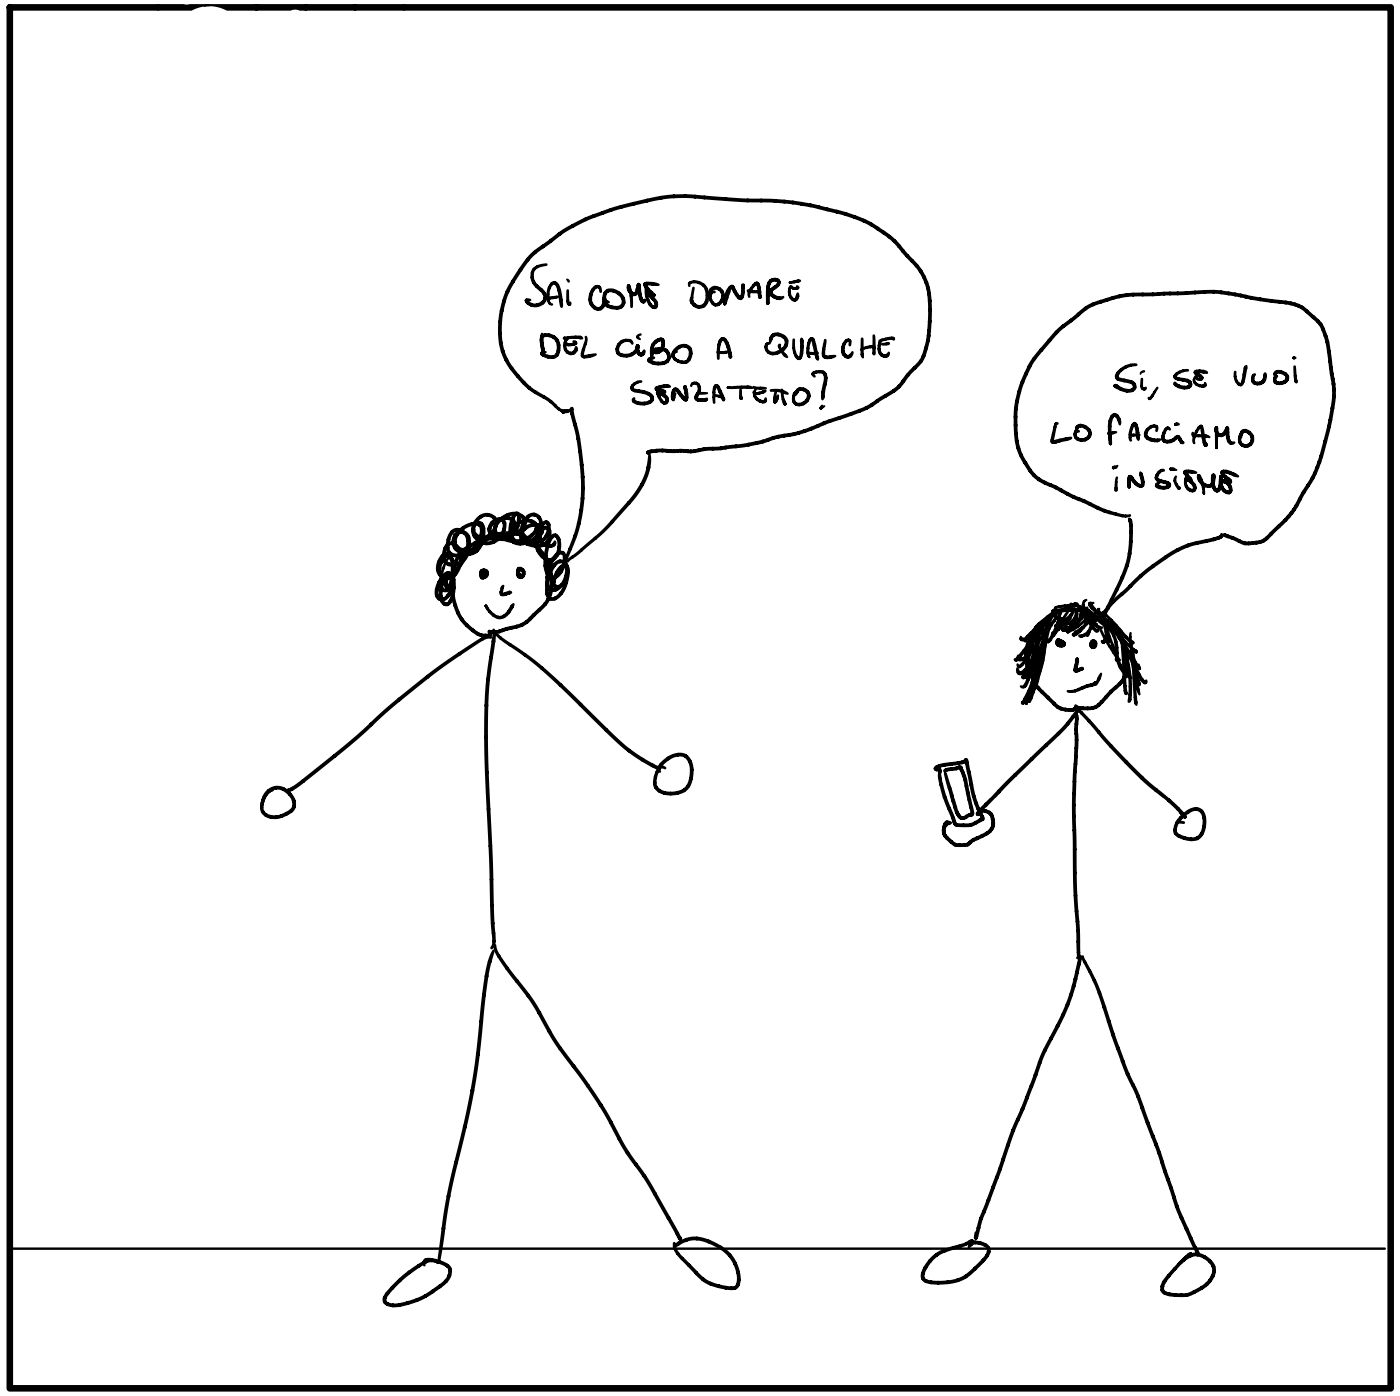
\includegraphics[width=0.3\textwidth]{Storyboard/task1-img II versione/t1.1.png} &
        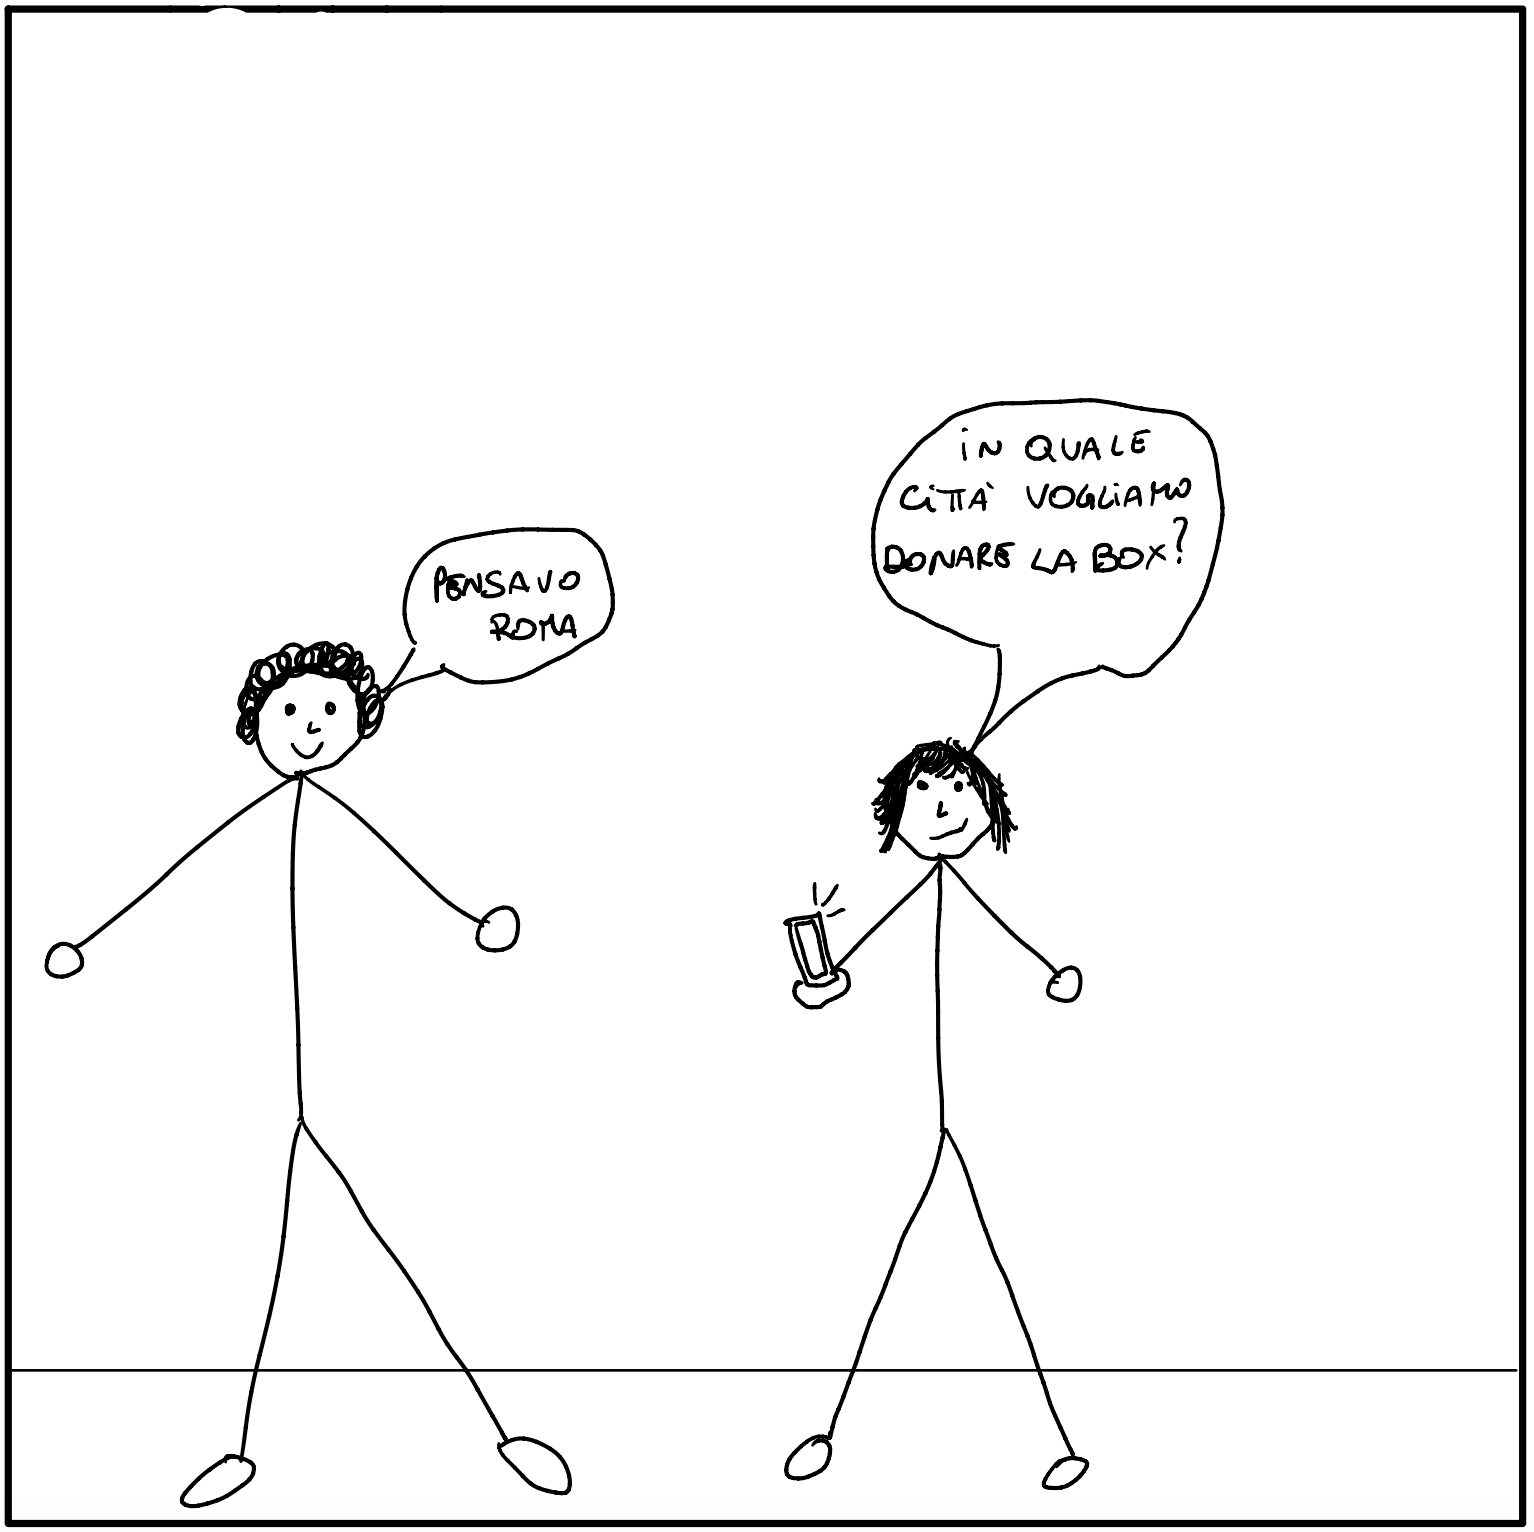
\includegraphics[width=0.3\textwidth]{Storyboard/task1-img II versione/t1.2.png} &
        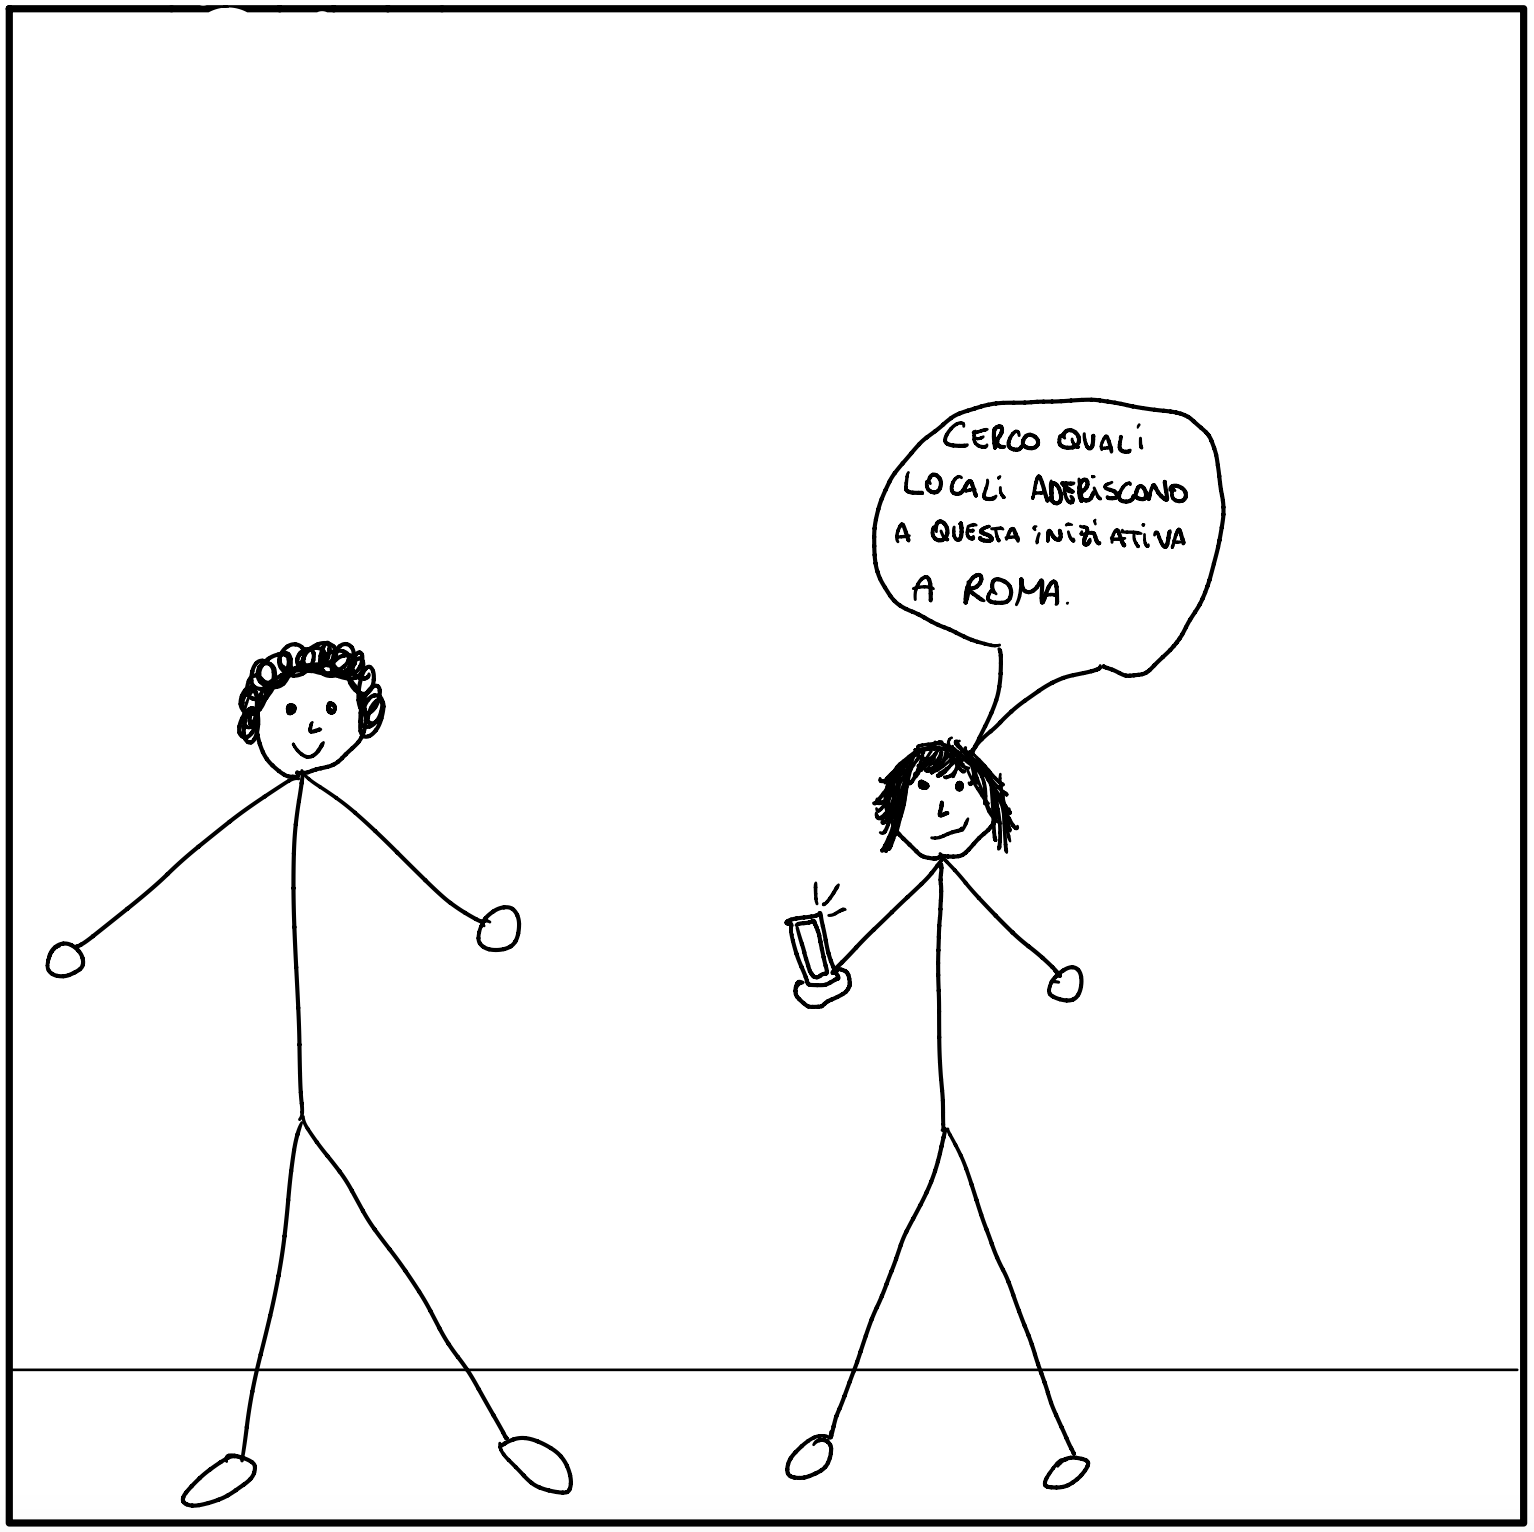
\includegraphics[width=0.3\textwidth]{Storyboard/task1-img II versione/t1.3.png} \\
        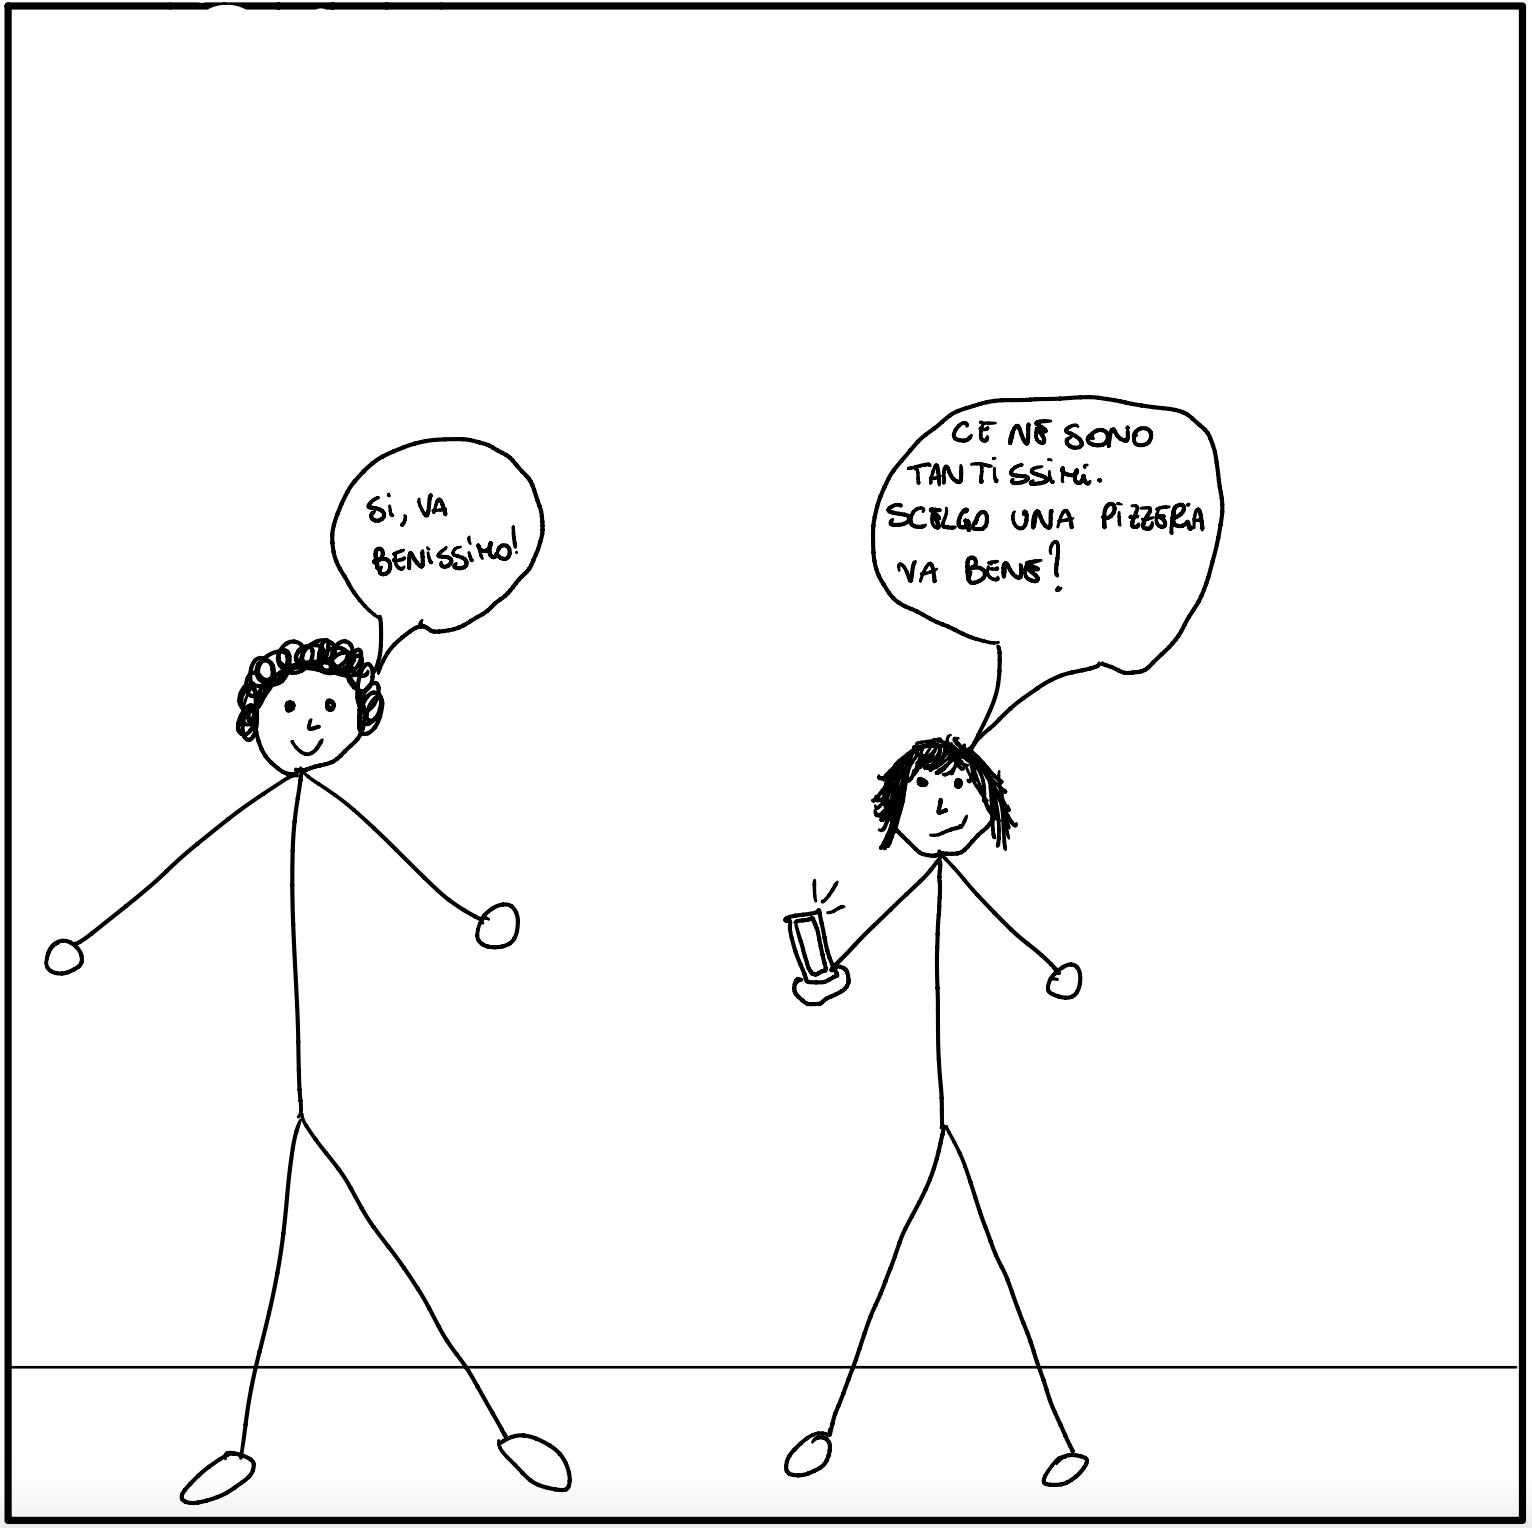
\includegraphics[width=0.3\textwidth]{Storyboard/task1-img II versione/t1.4.png} &
        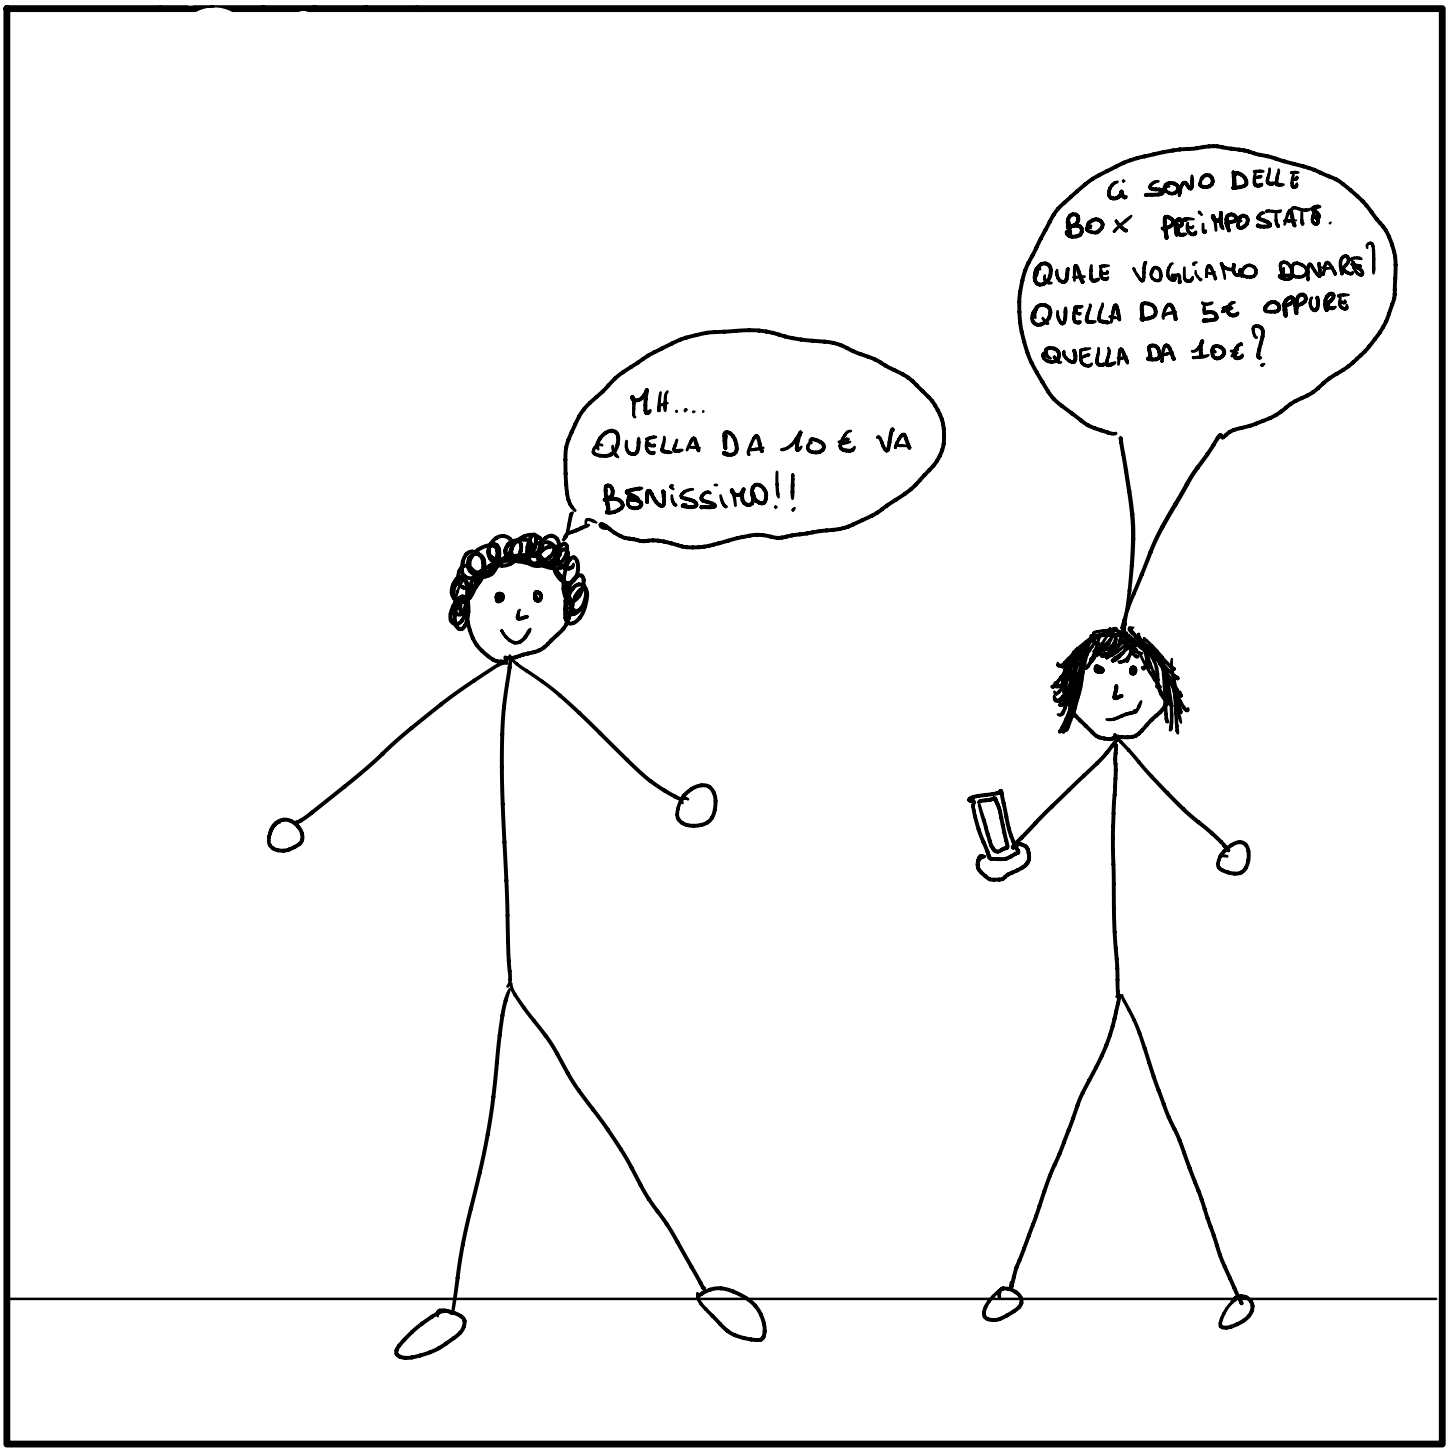
\includegraphics[width=0.3\textwidth]{Storyboard/task1-img II versione/t1.5.png} &
        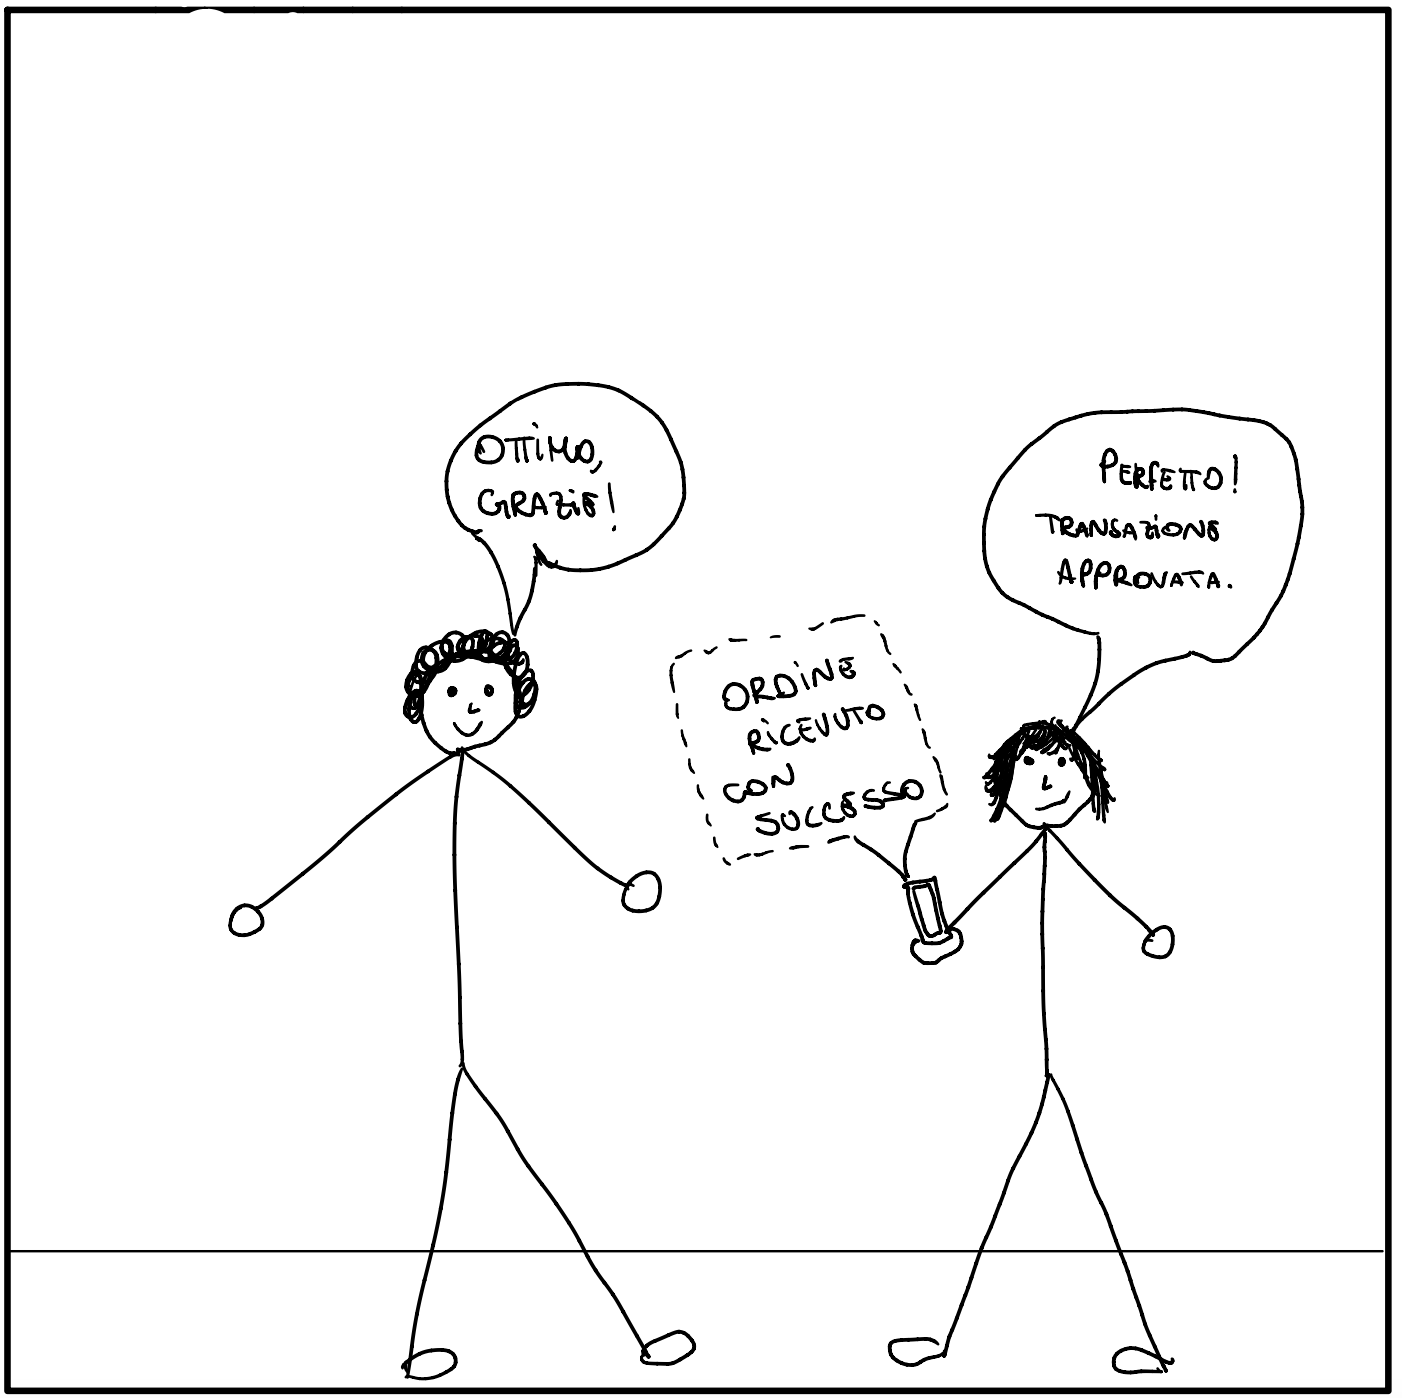
\includegraphics[width=0.3\textwidth]{Storyboard/task1-img II versione/t1.6.png} \\
    \end{tabular}
    \label{fig:task1}
\end{figure}


\newpage
\subsection{Task 2}
L'utente annuncia la disponibilità di cibo invenduto da regalare/vendere, fornendo informazioni/foto sul cibo e la quantità disponibile.
\begin{figure}[H]
    \centering
    \begin{tabular}{ccc}
        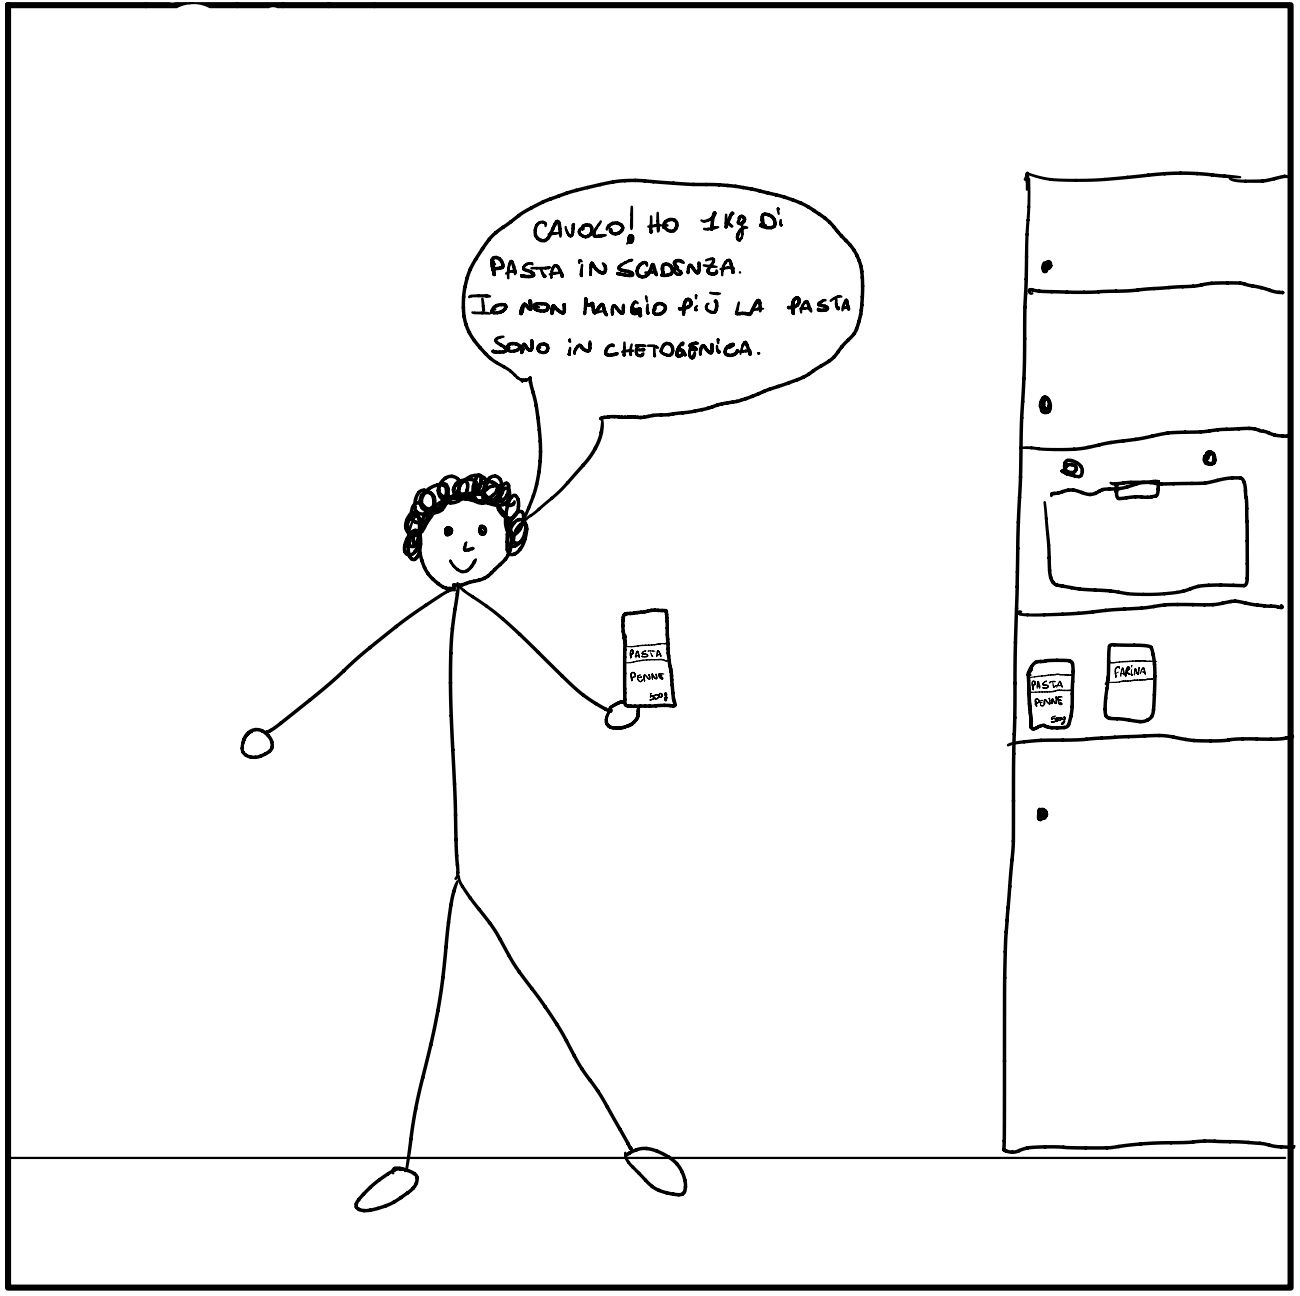
\includegraphics[width=0.3\textwidth]{Storyboard/task2-img II versione/t2.1.png} &
        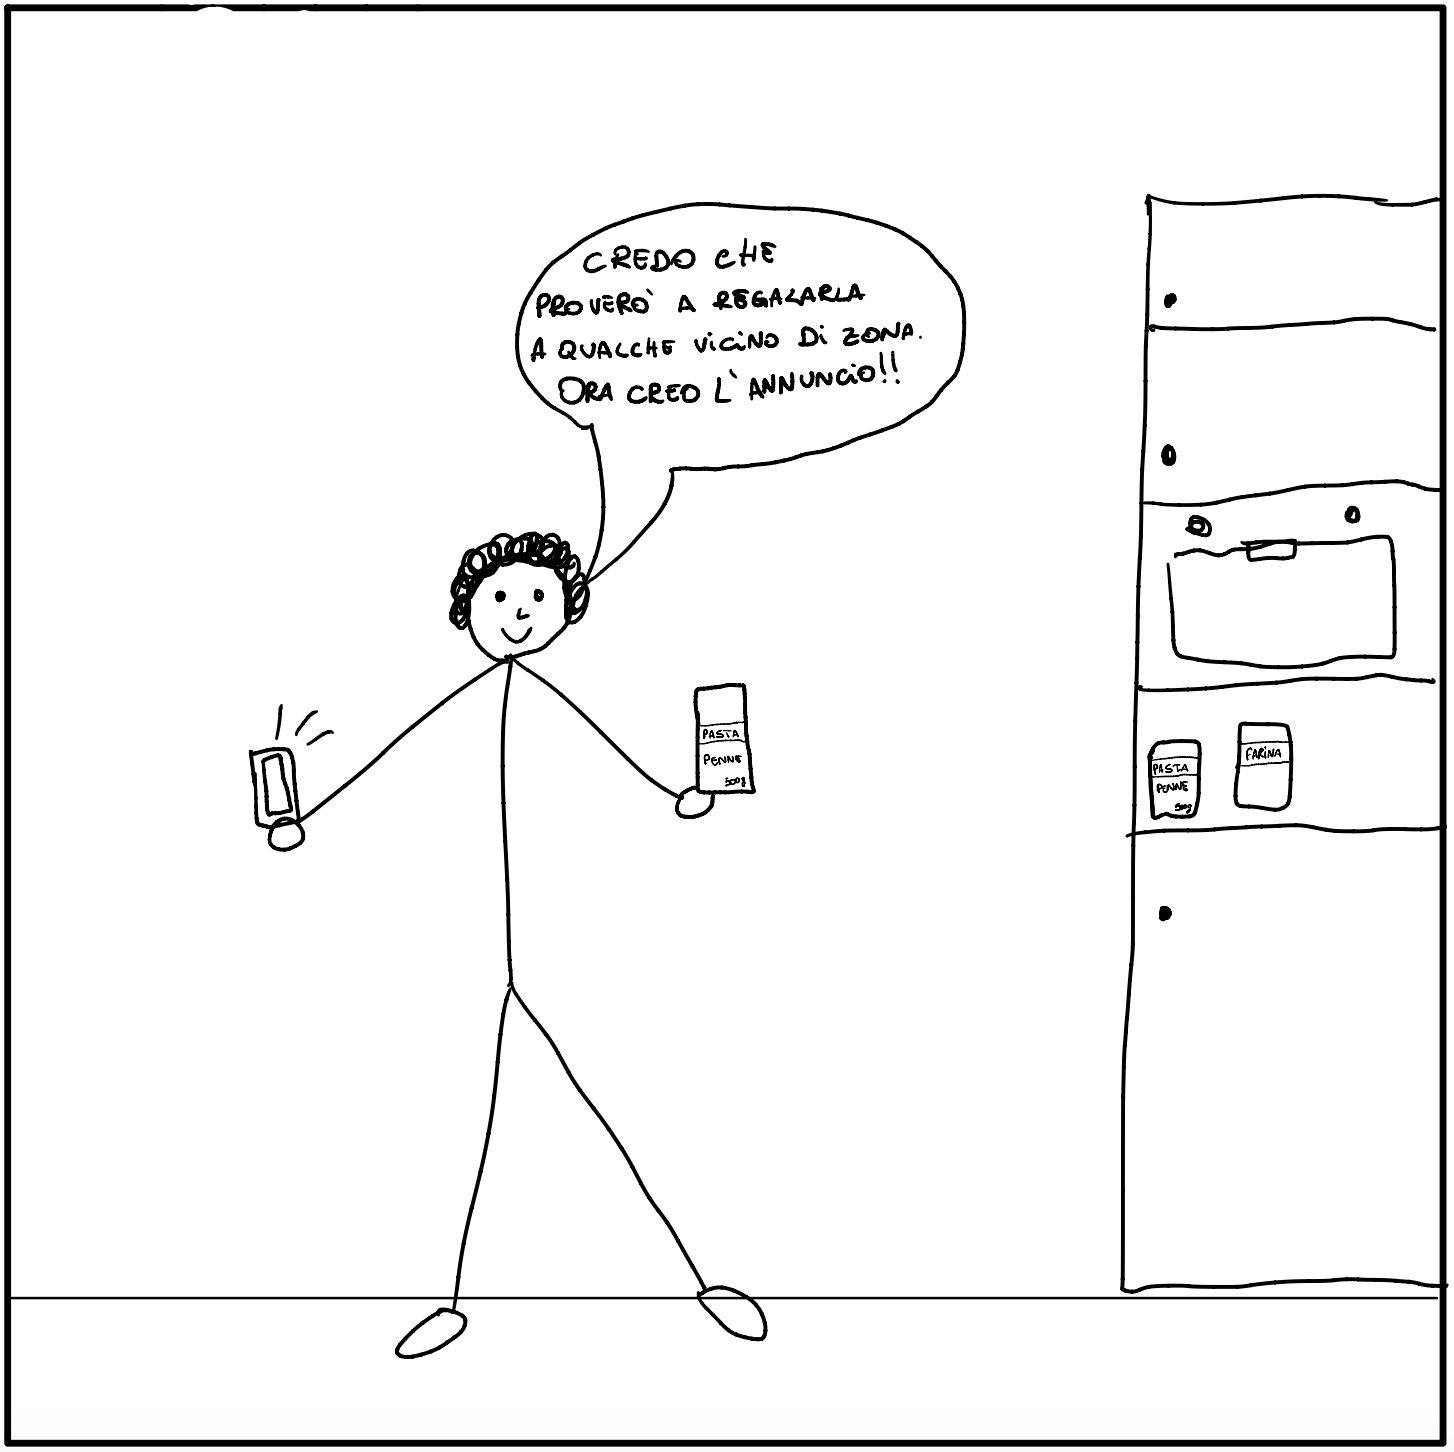
\includegraphics[width=0.3\textwidth]{Storyboard/task2-img II versione/t2.2.png} &
        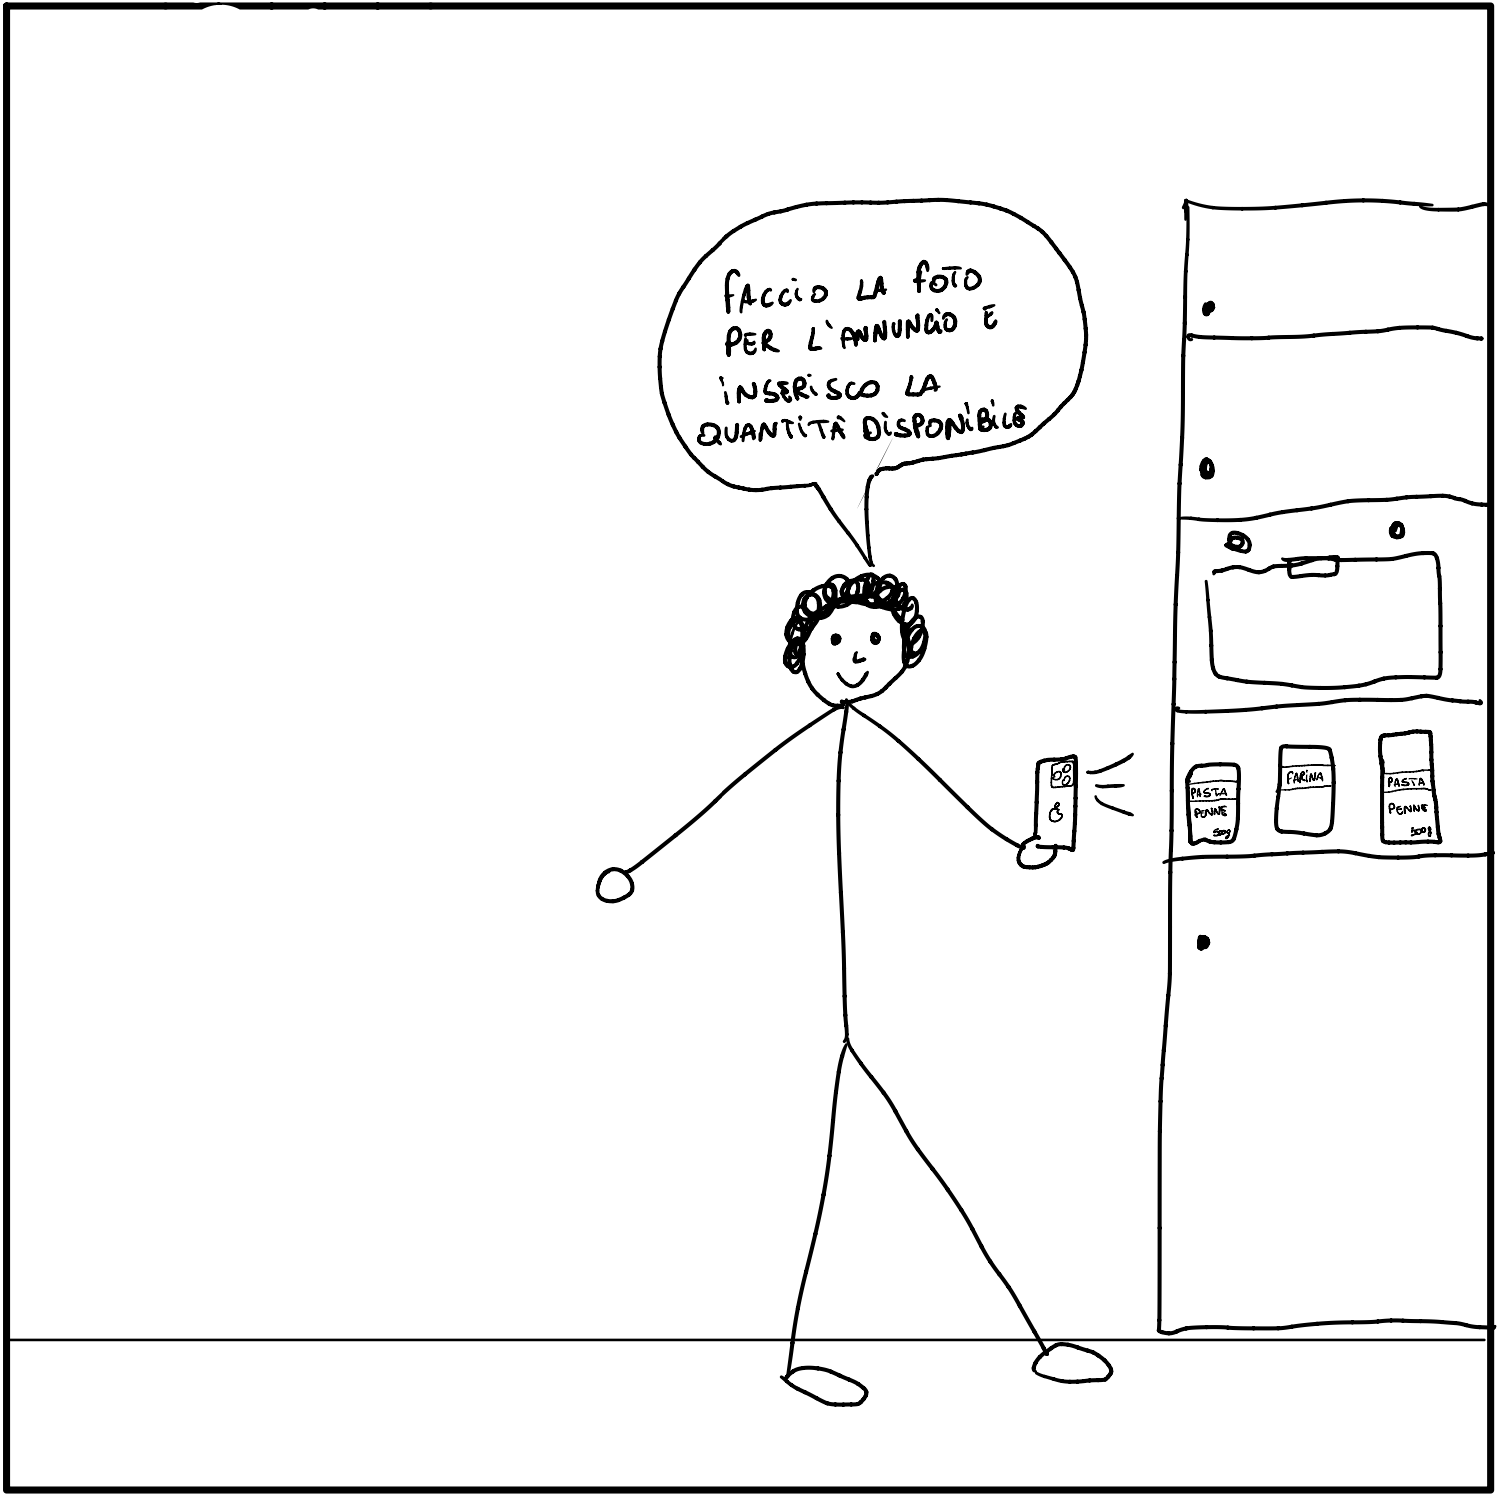
\includegraphics[width=0.3\textwidth]{Storyboard/task2-img II versione/t2.3.png} \\
        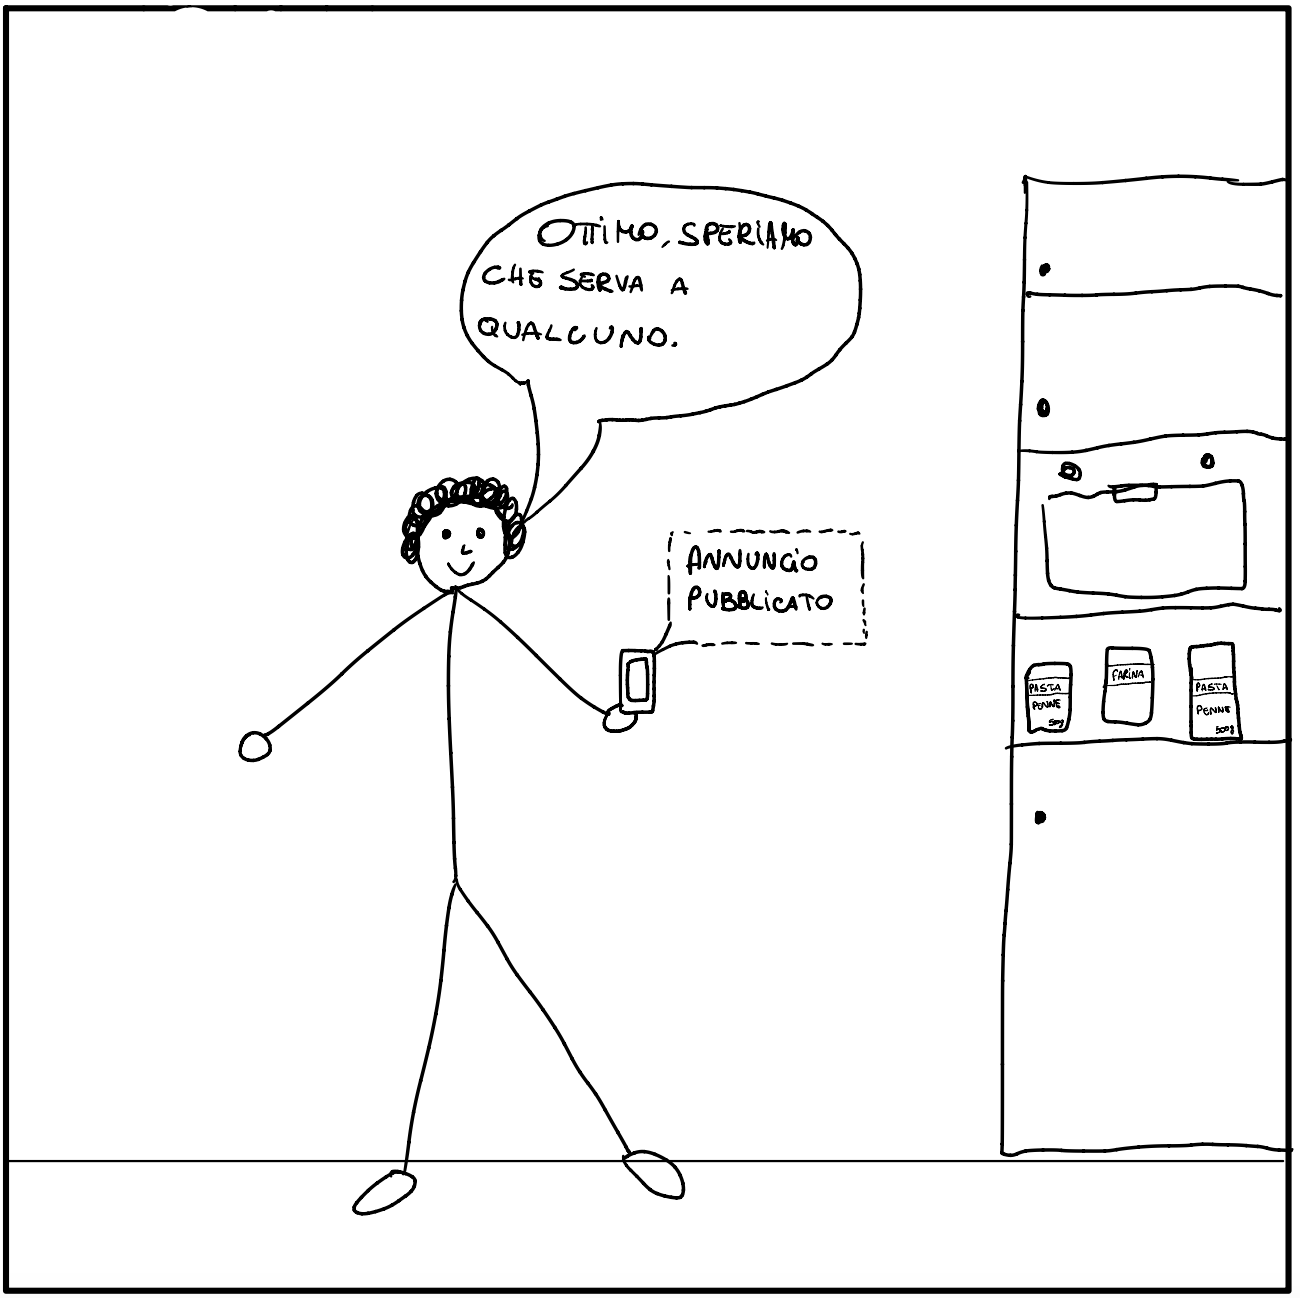
\includegraphics[width=0.3\textwidth]{Storyboard/task2-img II versione/t2.4.png} & & \\
    \end{tabular}
    \label{fig:task2}
\end{figure}

\newpage
\subsection{Task 3}
L'utente filtra i risultati dei locali per Città e fascia oraria di ritiro/consegna del cibo invenduto, sceglie un locale e acquista una box di cibo invenduto con consegna.
\begin{figure}[H]
    \centering
    \begin{tabular}{ccc}
        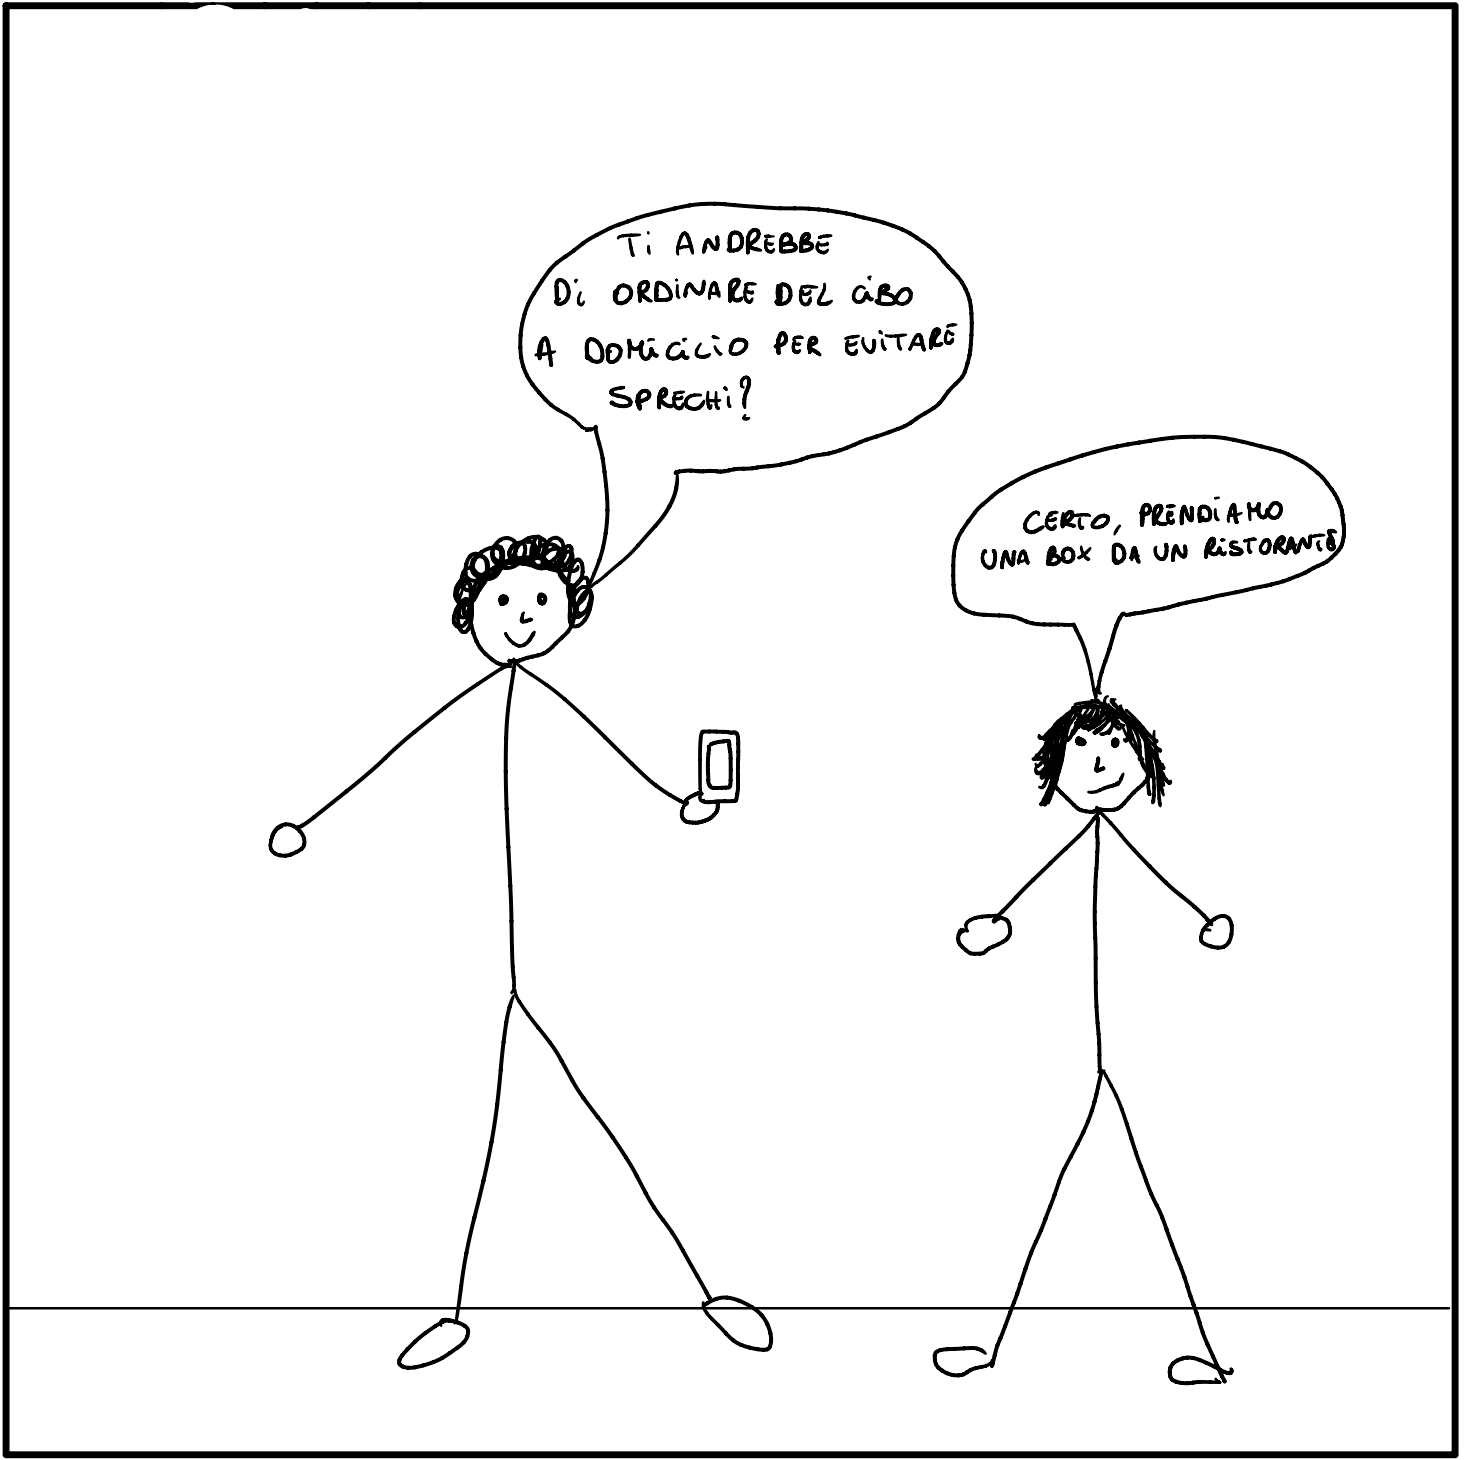
\includegraphics[width=0.3\textwidth]{Storyboard/task3-img/t3.1.png} &
        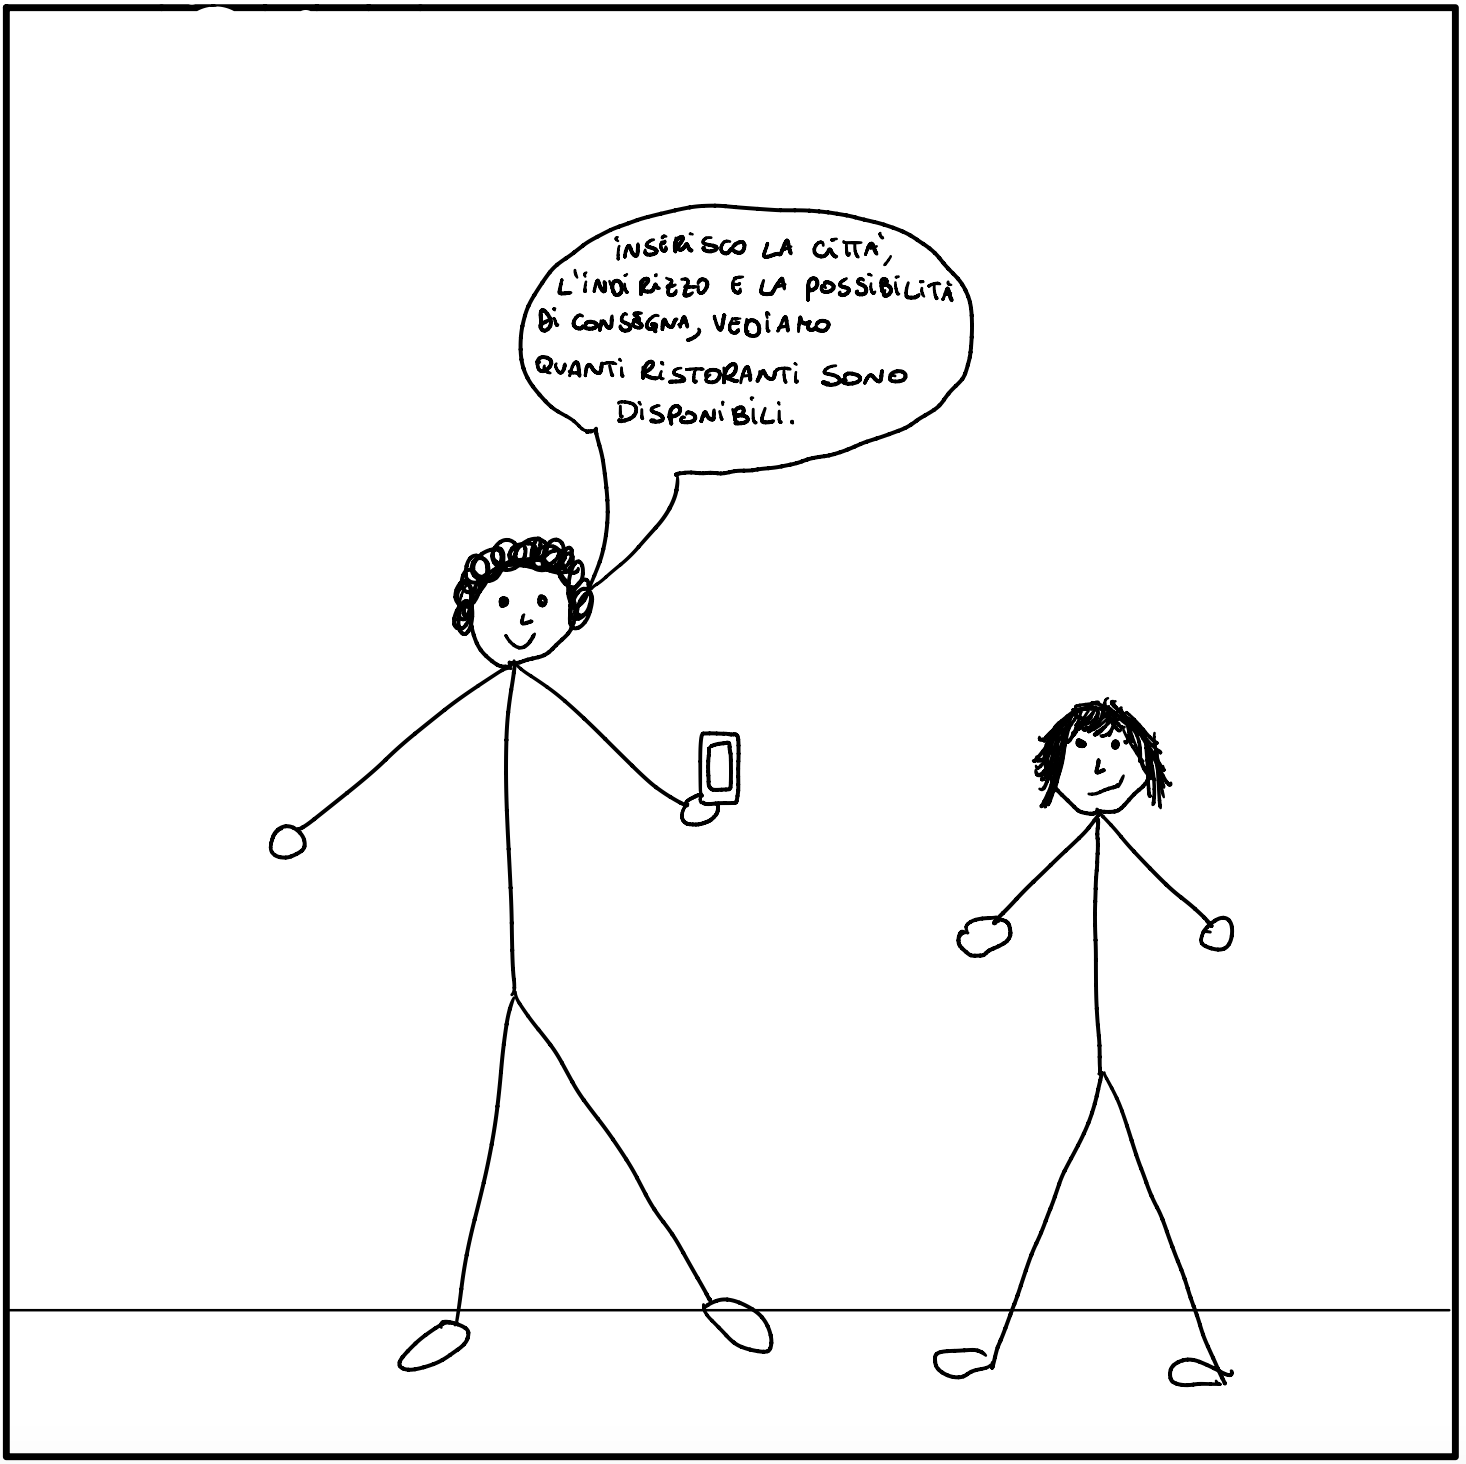
\includegraphics[width=0.3\textwidth]{Storyboard/task3-img/t3.2.png} &
        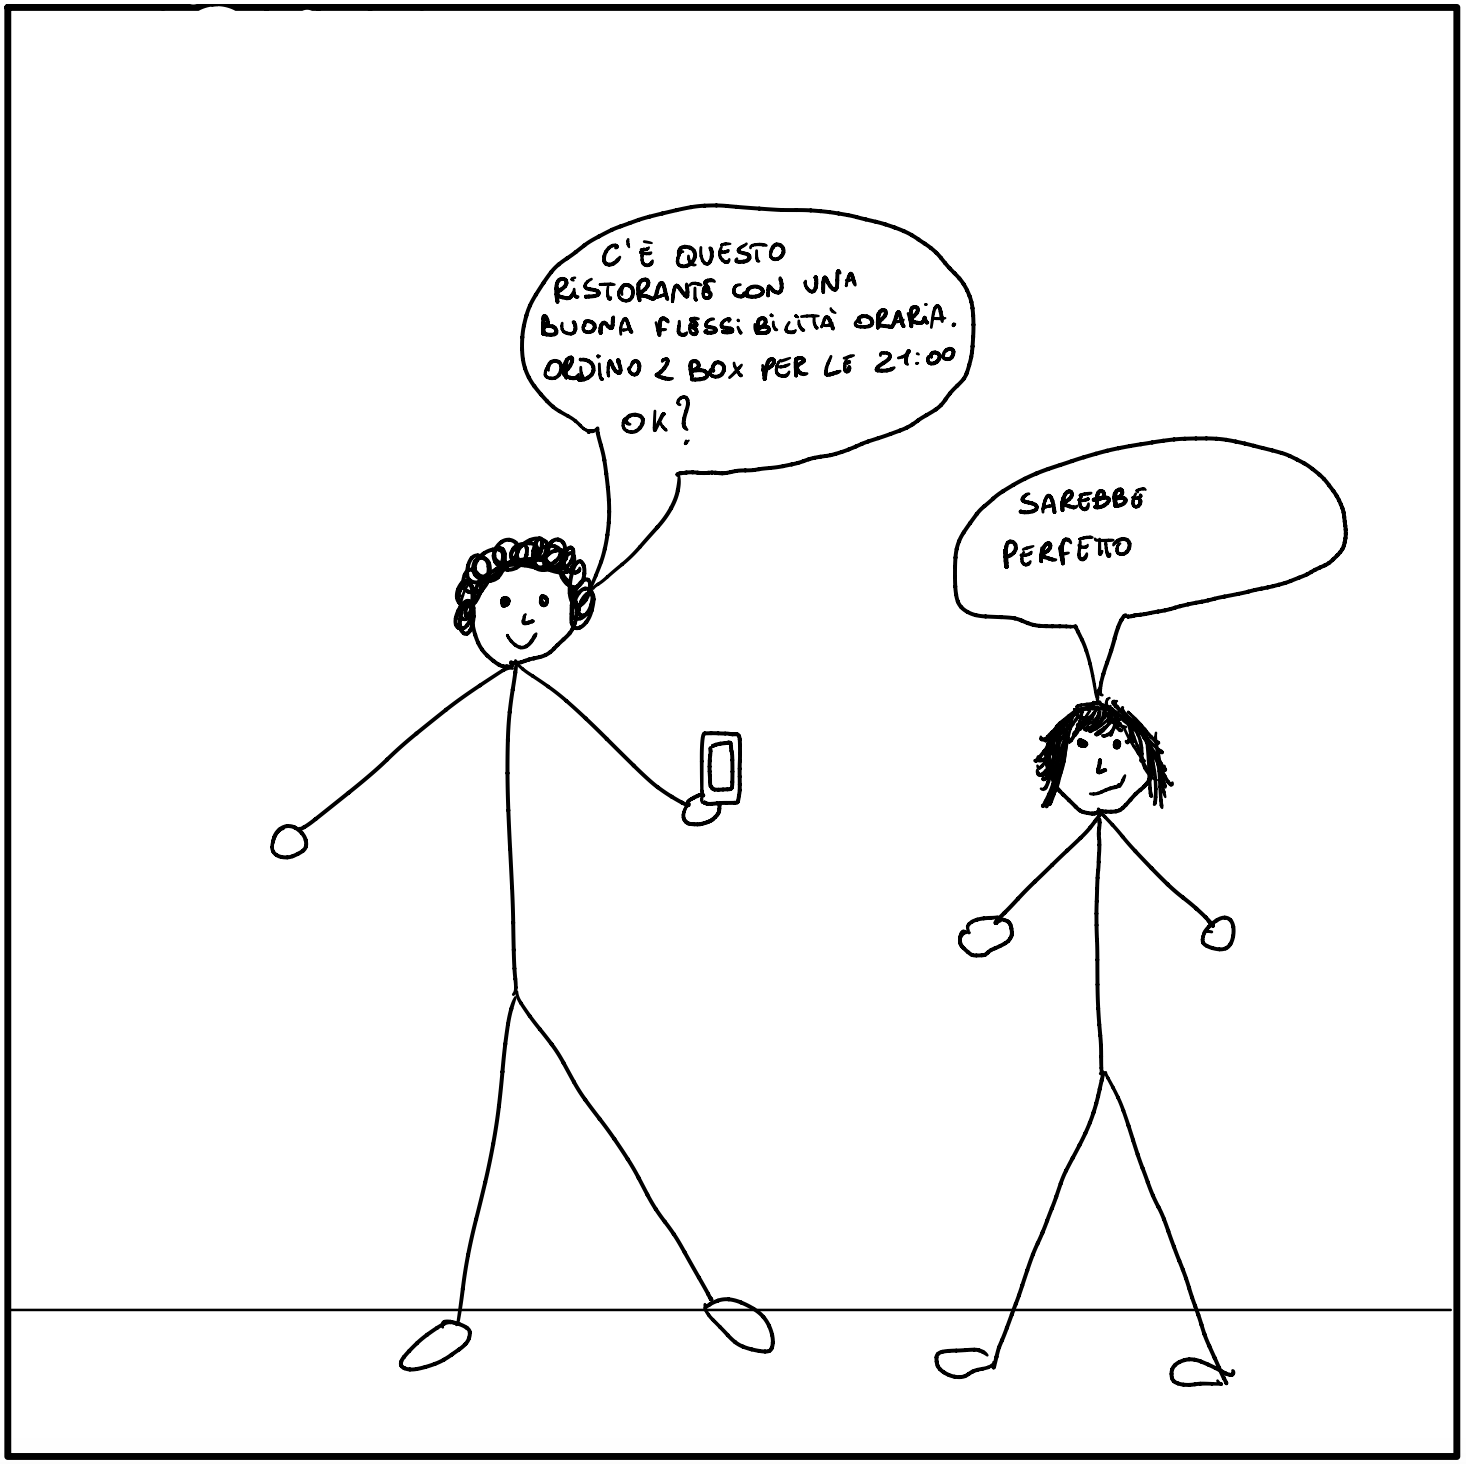
\includegraphics[width=0.3\textwidth]{Storyboard/task3-img/t3.3.png} \\
        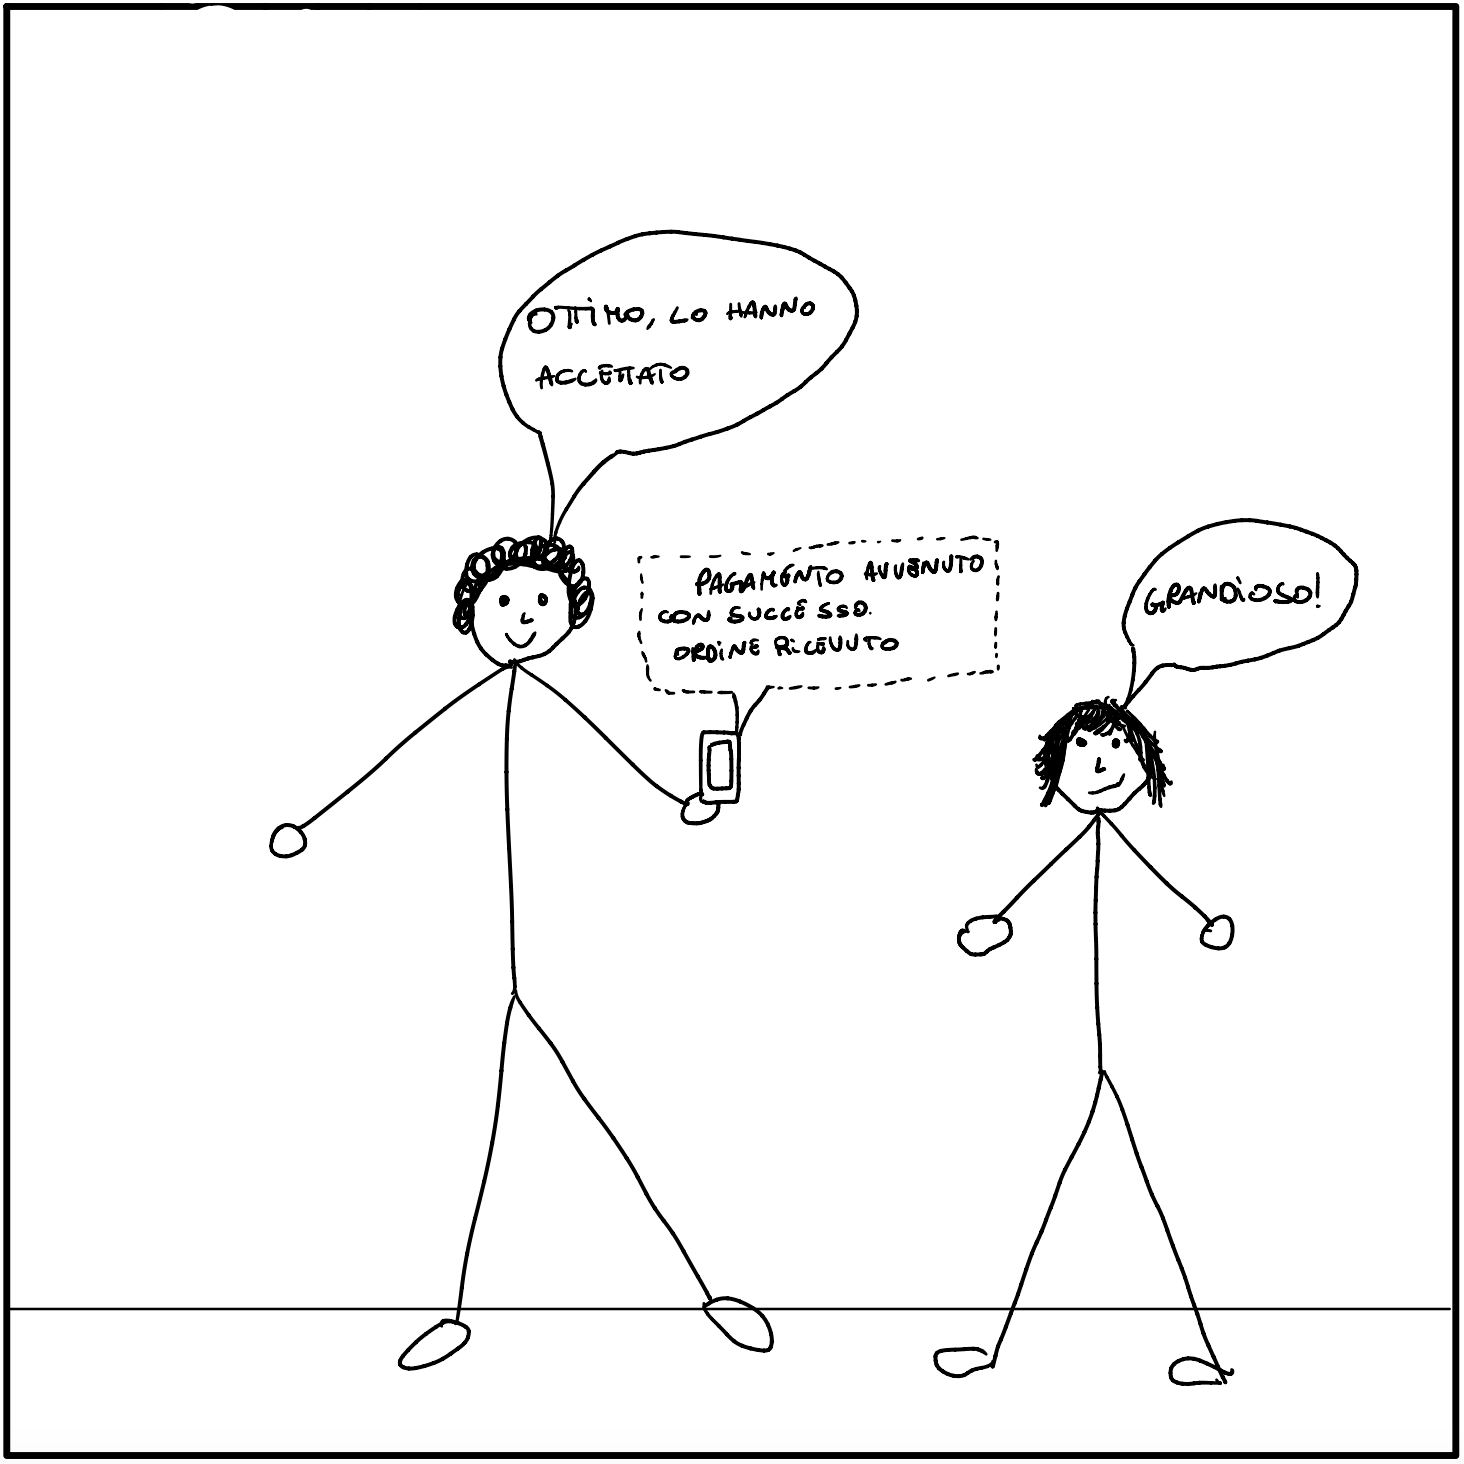
\includegraphics[width=0.3\textwidth]{Storyboard/task3-img/t3.4.png} & & \\
    \end{tabular}
    \label{fig:task2}
\end{figure}

\section{Prototyping}

Per quanto riguarda il prototyping, è stato utilizzato un approccio di tipo \textit{\textbf{evolutivo}}, ovvero il prototipo iniziale è stato utilizzato come base per la creazione di prototipi successivi.

In tutte le versioni dei prototipi, sono stati seguiti gli standard per IOS (Human Interface Guidelines), minimizzando l'utilizzo di campi obbligatori e mantenendo un design pulito e intuitivo.
C'è la presenza di una vista modale, nella schermata di conferma del pagamento.
La navigation bar è presente in tutte le schermate, con la possibilità di tornare alla home in qualsiasi momento.

\subsection{Paper prototype}

\paragraph{Prima versione}
\mbox{}
\newline
Il primo prototipo cartaceo, implementa tutti e tre i task identificati in precedenza.
I test sono stati effettuati con il metodo \textbf{Cooperative Evaluation}, ovvero l'utente e l'esperto hanno lavorato insieme per valutare il prototipo, questo perché gli utenti non avevano molta esperienza con questo tipo di test e hanno preferito lavorare insieme all'esperto.
Successivamente ai test effettuati con gli utenti e un esperto, si sono individuati i seguenti problemi:
\begin{itemize}
    \item \textbf{Task 1:} L'utente/l'esperto non riesce a determinare quale sia l'icona dei filtri generici e i filtri per la mappa, andando intuitivamente sul bottone che gestisce la visualizzazione dei locali (se sotto forma di lista o direttamente sulla mappa). Un altro problema risulta essere la sezione per le box disponibili per le donazioni, intuitivamente risalta all'occhio dell'utente la sezione per le box disponibili per l'acquisto (non per le donazioni).
    \item \textbf{Task 2:} Qui la maggior parte dei dubbi si riscontrano nell'inserimento del prezzo, non sembra molto chiaro per gli utenti/l'esperto come trattare la sezione del prezzo in caso si volesse regalare l'articolo e quindi non inserendo alcun prezzo, trovando comunque una soluzione al problema.
    \item \textbf{Task 3:} I problemi in questo caso sono simili al primo task (come filtrare i risultati), tranne che per la sezione di pagamento, dove all'utente/esperto non è chiaro se premere "paga ora" oppure "paga al ritiro/consegna", inoltre non è richiesto inserire l'indirizzo di spedizione, dando per scontato che sia stato già inserito in fase di filtraggio dei risultati.
\end{itemize}
L'esperto ha inoltre consigliato di cambiare il colore degli interruttori quando non sono attivi, ovvero di eliminare il colore, in modo tale da evitare di confondere gli utenti e farli pensare che siano attivi.

\paragraph{Seconda versione}
\mbox{}
\newline
Anche in questo caso i test sono stati effettuati con il metodo \textbf{Cooperative Evaluation}, avendo visto un riscontro positivo nell'utilizzo di questa tecnica nella prima versione.
Nella seconda versione del prototipo cartaceo, sono stati apportati i cambiamenti necessari per risolvere i problemi riscontrati nella prima versione, ovvero:
\begin{itemize}
    \item \textbf{Task 1:} E' stata eliminata la sezione di visualizzazione dei locali (in modalità lista o modalità mappa) e unificata l'icona per i filtri generici e i filtri per la mappa. La scelta per le box disponibili per le donazioni è stata gestita in modo tale da obbligare l'utente a leggere la descrizione delle sezioni, in modo tale da capire quale sezione faccia al suo caso.
    \item \textbf{Task 2:} Non sono state apportate modifiche importanti tranne che per la schermata iniziale, che segue lo stesso principio della modifica fatta per il task 1. 
    \item \textbf{Task 3:} Per la parte iniziale del task sono state effettuate le stesse modifiche del task 1, mentre per la parte finale è stato aggiunto un campo per scegliere se farsi consegnare la box o ritirarlo in loco, in modo tale da evitare confusione all'utente sul pulsante da premere per il pagamento, nel caso di consegna a domicilio è stato aggiunto un campo per inserire l'indirizzo di spedizione.
\end{itemize}

In questo caso complessivamente il prototipo cartaceo è stato migliorato, risolvendo quasi completamente i problemi riscontrati nella prima versione.

Un problema è stato riscontrato nel \textbf{task 3}, dove l'utente/l'esperto si chiede come mai gli venga richiesto l'indirizzo di consegna nonostante lo abbia inserito durante la fase di filtraggio dei risultati.
Anche in questo caso per il \textbf{task 2} è stato riscontrato lo stesso problema, ma l'utente/l'esperto ha risolto il problema da solo, ipotizzando che inserire tutti zeri nel campo dell'importo, potesse significare che l'articolo fosse gratuito.

L'esperto ha notato un problema sul flusso delle operazioni, l'esperto si chiede con quale ordine vanno eseguite le azioni (e.s. quale filtro utilizzare per primo), i prototipi sviluppati fino a questo punto obbligano a seguire un flusso di operazioni, senza lasciare la libertà all'utente di scegliere l'ordine delle azioni.

\subsection{High-fidelity prototype}

\paragraph{Prima versione}
\mbox{}
\newline
I prototipi ad alta fedeltà sono stati realizzati con Figma, un software di prototipazione online.

Link al prototipo: \href{https://www.figma.com/proto/xET26iTanAxBERu0jhT0FS/Task?node-id=0-1&t=yNOGB0vveNBLslKN-1}{"\textcolor{blue}{Task 1}"}, \href{https://www.figma.com/design/xET26iTanAxBERu0jhT0FS/Task?node-id=31-38&t=yNOGB0vveNBLslKN-1}{"\textcolor{blue}{Task 2}"}, \href{https://www.figma.com/proto/xET26iTanAxBERu0jhT0FS/Task?node-id=74-42&t=yNOGB0vveNBLslKN-1}{"\textcolor{blue}{Task 3}"}.

I test sono stati effettuati con il metodo \textbf{Thinking Aloud}, ovvero l'utente parla ad alta voce mentre esegue i task, in modo tale da permettere all'esperto di capire quali sono i problemi riscontrati dall'utente.
In questo caso è stato scelto questo approccio, data l'interattività del prototipo ad alta fedeltà, che consente all'utente una maggiore autonomia nello scegliere le azioni da eseguire.

Il primo prototipo ad alta fedeltà, implementa tutti e tre i task identificati in precedenza, fornendo però la possibilità di scegliere l'ordine delle azioni da eseguire, come consigliato dall'esperto nella fase precedente.
Successivamente ai test effettuati con gli utenti e un esperto, si sono individuati i seguenti problemi:
\begin{itemize}
    \item \textbf{Task 1:} L'utente/l'esperto non vede intuitiva la schermata dove deve scegliere tra le box disponibili per le donazioni o quelle disponibili solamente all'acquisto.
    \item \textbf{Task 2:} In questo caso l'utente/l'esperto sembra avere tutto chiaro, se non per una piccola esitazione nel cercare il bottone per pubblicare l'annuncio.
    \item \textbf{Task 3:} Anche in questo caso l'utente/l'esperto ha gli stessi problemi del primo task.
\end{itemize}

\paragraph{Seconda versione}
\mbox{}
\newline
Link al prototipo: \href{https://www.figma.com/proto/xET26iTanAxBERu0jhT0FS/Task?node-id=0-1&t=yNOGB0vveNBLslKN-1}{"\textcolor{blue}{Task 1}"}, \href{https://www.figma.com/design/xET26iTanAxBERu0jhT0FS/Task?node-id=31-38&t=yNOGB0vveNBLslKN-1}{"\textcolor{blue}{Task 2}"}, \href{https://www.figma.com/proto/xET26iTanAxBERu0jhT0FS/Task?node-id=74-42&t=yNOGB0vveNBLslKN-1}{"\textcolor{blue}{Task 3}"}.

Nella seconda versione del prototipo ad alta fedeltà, sono stati apportati i cambiamenti necessari per risolvere i problemi riscontrati nella prima versione, ovvero:
\begin{itemize}
    \item \textbf{Task 1:} E' stata ristrutturata la schermata in cui l'utente deve scegliere tra le box disponibili per le donazioni o quelle disponibili.
    \item \textbf{Task 2:} Non sono state apportate modifiche importanti tranne che per il bottone per la pubblicazione dell'annuncio, che è stato spostato in basso.
    \item \textbf{Task 3:} Per risolvere il problema in comune al task 1, è stata ristrutturata la schermata in cui l'utente deve scegliere tra le box disponibili per le donazioni o quelle disponibili.
\end{itemize}

In questo caso complessivamente il prototipo ad alta fedeltà è stato migliorato, risolvendo quasi completamente i problemi riscontrati nella prima versione.
Rimane un piccolo problema segnalato dall'esperto e uno segnalato da un utente, ovvero il bottone per l'inserimento dell'annuncio, che suggerisce di inserire completamente nella barra di navigazione in basso, così da mantenere un design più affine a quello di IOS e infine quello di inserire un tasto per tornare direttamente alla home, dato che la freccia in alto a sinistra non è molto intuitiva.

\paragraph{Terza versione}
\mbox{}
\newline
Link al prototipo: \href{https://www.figma.com/proto/xET26iTanAxBERu0jhT0FS/Task?node-id=0-1&t=yNOGB0vveNBLslKN-1}{"\textcolor{blue}{Task 1}"}, \href{https://www.figma.com/design/xET26iTanAxBERu0jhT0FS/Task?node-id=31-38&t=yNOGB0vveNBLslKN-1}{"\textcolor{blue}{Task 2}"}, \href{https://www.figma.com/proto/xET26iTanAxBERu0jhT0FS/Task?node-id=74-42&t=yNOGB0vveNBLslKN-1}{"\textcolor{blue}{Task 3}"}.

Nella terza versione del prototipo ad alta fedeltà, sono stati apportati i cambiamenti necessari per risolvere i problemi riscontrati nella seconda versione, ovvero:
\begin{itemize}
    \item \textbf{Task 1:} E' stato inserito un bottone per tornare alla home, in modo tale da rendere più intuitivo il ritorno alla schermata iniziale.
    \item \textbf{Task 2:} E' stato spostato il bottone per l'inserimento dell'annuncio completamente nella barra di navigazione in basso, in modo tale da mantenere un design più affine a quello di IOS.
    \item \textbf{Task 3:} E' stato inserito un bottone per tornare alla home, in modo tale da rendere più intuitivo il ritorno alla schermata iniziale.
\end{itemize}

Un cambiamento che prende tutti i task è stato quello di aggiungere il tasto per tornare alla home, in modo tale da rendere più intuitivo il ritorno alla schermata iniziale.

In questo caso complessivamente il prototipo ad alta fedeltà è stato migliorato, risolvendo completamente i problemi riscontrati nella seconda versione.






\end{document}
